% -- Anfang Präambel
\documentclass[german,  % Standardmäßig deutsche Eigenarten, englisch -> english
parskip=full,  % Absätze durch Leerzeile trennen
%bibliography=totoc,  % Literatur im Inhaltsverzeichnis (ist unüblich)
%draft,  % TODO: Entwurfsmodus -> entfernen für endgültige Version
]{scrartcl}
\usepackage[utf8]{inputenc}  % Kodierung der Datei
\usepackage[T1]{fontenc}  % Vollen Umfang der Schriftzeichen
\usepackage[ngerman]{babel}  % Sprache auf Deutsch (neue Rechtschreibung)

% Mathematik und Größen
\usepackage{amsmath}
\usepackage[locale=DE,  % deutsche Eigenarten, englisch -> US
separate-uncertainty,  % Unsicherheiten seperat angeben (mit ±)
]{siunitx}
\usepackage{physics}  % Erstellung von Gleichungen vereinfachen
\usepackage{yfonts}  % Frakturschrift für Real- und Imaginärteil komplexer Größen

\usepackage{graphicx}  % Bilder einbinden \includegraphics{Pfad/zur/Datei(ohne Dateiendung)}

% Gestaltung
%\usepackage{microtype}  % Mikrotypographie (kann man am Ende verwenden)
\usepackage{booktabs}  % schönere Tabellen
%\usepackage[toc]{multitoc}  % mehrspaltiges Inhaltsverzeichnis
\usepackage{csquotes}  % Anführungszeichen mit \enquote
\usepackage{caption}  % Anpassung der Bildunterschriften, Tabellenüberschriften
\usepackage{subcaption}  % Unterabbildungen, Untertabellen, …
\usepackage{enumitem}  % Listen anpassen
\setlist{itemsep=-10pt}  % Abstände zwischen Listenpunkten verringern

% Manipulation des Seitenstils
\usepackage{scrpage2}
% Kopf-/Fußzeilen setzen
\pagestyle{scrheadings}  % Stil für die Seite setzen
\clearscrheadings  % Stil zurücksetzen, um ihn neu zu definieren
\automark{section}  % Abschnittsnamen als Seitenbeschriftung verwenden
\ofoot{\pagemark}  % Seitenzahl außen in Fußzeile
\ihead{\headmark}  % Seitenbeschriftung mittig in Kopfzeile
\setheadsepline{.5pt}  % Kopzeile durch Linie abtrennen

\usepackage[hidelinks]{hyperref}  % Links und weitere PDF-Features

% TODO: Titel und Autor, … festlegen
\newcommand*{\titel}{Beta-Zerfall}
\newcommand*{\autor}{Tom Drechsler, Konstantin Schmid}
\newcommand*{\abk}{BE}
\newcommand*{\betreuer}{Christian Wiel}
\newcommand*{\messung}{7. Februar 2020}
\newcommand*{\ort}{ASB/414}

\hypersetup{pdfauthor={\autor}, pdftitle={\titel}}  % PDF-Metadaten setzen

\addto{\captionsngerman}{
\renewcommand*{\figurename}{Abb.}
}
\addto{\captionsngerman}{
\renewcommand*{\tablename}{Tab.}
}


% automatischen Titel konfigurieren
\titlehead{Fortgeschrittenen-Praktikum \abk \hfill TU Dresden}
\subject{Versuchsprotokoll}
\title{\titel}
\author{\autor}
\date{\begin{tabular}{ll}
Protokoll: & \today\\
Messung: & \messung\\
Ort: & \ort\\
Betreuer: & \betreuer\end{tabular}}

% -- Ende Präambel
\usepackage{upgreek}



\begin{document}
\begin{titlepage}
\maketitle  % Titel setzen
\tableofcontents  % Inhaltsverzeichnis
\end{titlepage}

% Text Anfang
\section{Aufgabenstellung und Versuchsziel}
Die \(\beta\)-Umwandlung gehört neben \(\alpha\)-Zerfällen und \(\gamma\)-Übergängen zu den drei grundlegenden Arten von Kernstrahlung. In diesem Versuch sollen Betaspektren für die Nuklide $^{137}_{\ 55}\text{Cs}$ und \(^{85}_{36}\mathrm{Kr}\) aufgenommen werden. Bei beiden Nukliden handelt es sich um \(\beta^{-}\)-Strahler, die zudem ein charakteristisches \(\gamma\)-Spektrum sowie innere Konversion aufweisen. Die Analyse der verschiedenen Bestandteile des Spektrums ist ein Schwerpunkt dieser Arbeit, da sich hierbei wesentliche Merkmale der \(\beta\)-Strahlung studieren lassen. \\
Neben der Analyse von Spektren ist auch der experimentelle Nachweis der Strahlung von Interesse. Die Energieabgabe der \(\beta\)-Teilchen erfolgt überwiegend durch Stöße mit Elektronenhüllen und Bremsstrahlung. Im zweiten Versuchsteil soll daher der Energieverlust beim Durchdringen von unterschiedlich dicken Schichten aus Papier oder Aluminium über die diskreten Linien der Konversionselektronen untersucht werden.
\\\\
Insgesamt gliedert sich der Versuch in folgende Teilaufgaben:
\begin{itemize}
\item Aufnahme und Diskussion des charakteristischen $\gamma$-Untergrundes der Nuklide $^{137}_{ \ 55}\text{Cs}$ und \(^{85}_{36}\mathrm{Kr}\)
\item Aufnahme und Diskussion der $\beta$-Spektren von $^{137}_{\ 55}\text{Cs}$ und \(^{85}_{36}\mathrm{Kr}\)
\item Energiekalibrierung und Bestimmung der Auflösungsgrenze des Spektrometers
\item Bestimmung der Grenzenergien der $\beta$-Spektren von $^{137}_{ \ 55}\text{Cs}$ und \(^{85}_{36}\mathrm{Kr}\)
\item Untersuchung der Wechselwirkung von $\beta$-Strahlung mit Materie
\end{itemize}

\section{Theoretische Grundlagen}
\subsection{$\beta$-Umwandlung}
Die $\beta$-Umwandlung ist eine Form radioaktiver Umwandlung. Dabei können $\beta^-$- und $\beta^+$-Umwandlung unterschieden werden:
\begin{align*}
&\beta^+:\ p \rightarrow n + e^+ + \nu_e \\
&\beta^-:\ n \rightarrow p + e^- + \bar{\nu}_e.
\end{align*}
Dabei ist zu beachten, dass sich ein freies Neutron spontan umwandelt (\(\tau_{\mathrm{1/2}} = 610.1\,\mathrm{s}\)) wogegen das freie Proton stabil ist. Die \(\beta^{+}\)-Umwandlung des Protons in ein Neutron erfolgt nur im Atomkern. Für den Kern ergeben sich dann folgende Reaktionsgleichungen für die \(\beta\)-Umwandlungen:
\begin{align*}
&\beta^+:\ ^{A}_{Z}X \rightarrow \ ^{A}_{Z-1}Y + e^- + \nu_e \\
&\beta^-:\ ^{A}_{Z}X \rightarrow \ ^{A}_{Z+1}Y + e^- + \bar{\nu}_e.
\end{align*}
Die Vermittlung erfolgt bei beiden Prozessen über die schwache Wechselwirkung. Jeweils eines der drei Quarks im Proton bzw. im Neutron wechselt sein Flavour unter Emission eines virtuellen \(W\)-Bosons. Dieses zerfällt dann in ein ein Elektron oder Positron sowie ein Antineutrino bzw. Neutrino. Die Vorgänge lassen sich sehr anschaulich an einem Feynman-Diagramm nachvollziehen, wie in Abb. 1 und Abb. 2 dargestellt. \\\\
\begin{minipage}{0.48\textwidth}
\begin{flushleft}
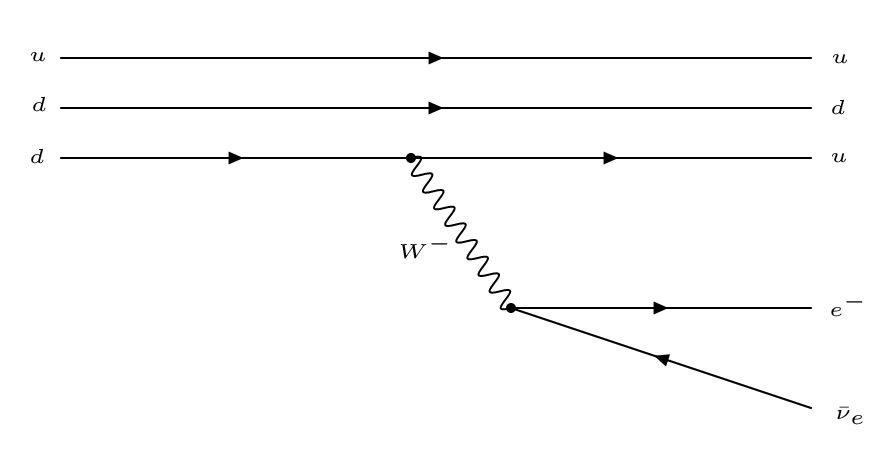
\includegraphics[width=1\textwidth]{/home/tom/BE/Beta_Minus.png}
\captionof{figure}{Feynmandiagramm des \(\beta^+\)-Zerfalls.}
\end{flushleft}
\end{minipage}
\begin{minipage}{0.04\textwidth}\centering
\[\ \ \]
\end{minipage}
\begin{minipage}{0.48\textwidth}
\begin{flushright}
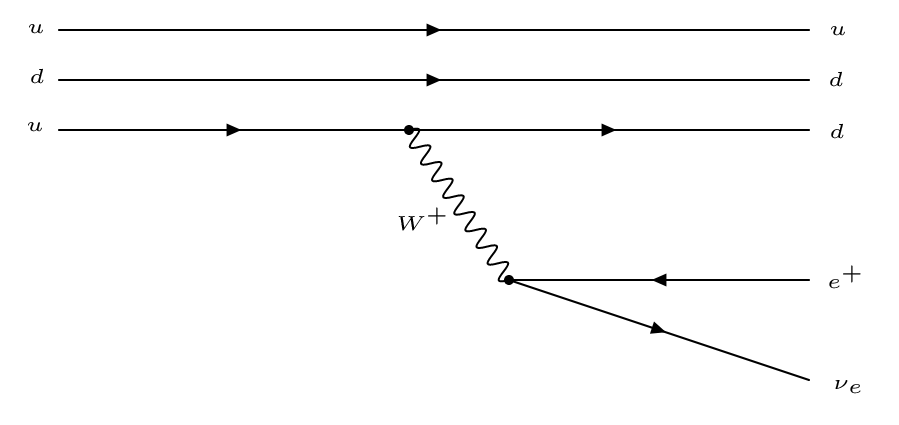
\includegraphics[width=1\textwidth]{/home/tom/BE/Beta_Plus.png}
\captionof{figure}{Feynmandiagramm des \(\beta^-\)-Zerfalls.}
\end{flushright}
\end{minipage} \\\\
Je nach Spineinstellung von Elektron und Neutrino werden 2 Fälle unterschieden:
\begin{itemize}
\item Fermi-Übergänge: Spins antiparallel ($S=0$)
\item Gamow-Teller-Übergänge: Spins parallel ($S=1$)
\end{itemize}
Die Aufteilung des Kernspins $I_I$ des Ausgangskerns erfolgt dann je nach Übergang nach folgenden Gleichungen:
\begin{align*}
\text{Fermi}: & \ I_F = I_I +L \\
\text{Gamow-Teller}: & \ I_F = I_I + L + 1.
\end{align*}
Dabei bezeichnet $I_F$ den Kernspin des Tochterkerns und $L$ den Drehimpuls des Elektron-Neutrino-Paares. Es kann nun eine Änderung der Parität $\Delta \pi$ betrachtet werden:
\begin{align*}
\Delta \pi = (-1)^L.
\end{align*}
Für $\Delta \pi = 1$ haben Mutter- und Tochterkern die gleiche Parität. Für $\Delta \pi = -1$ findet eine Paritätsänderung statt. Daraus ergeben sich Auswahlregeln, welche in Abb. 3 zu finden sind.
\newpage
\begin{figure}[h!]
\centering
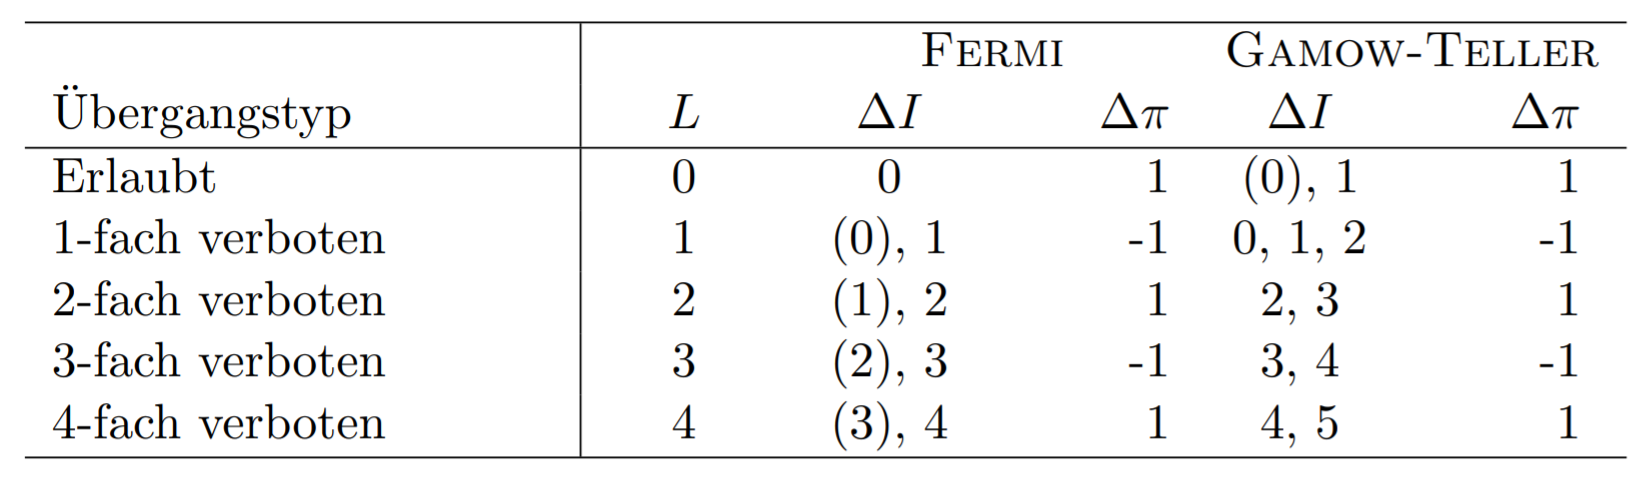
\includegraphics[width=\textwidth]{auswahlregeln}
\caption{Auswahlregeln für $\beta$-Übergänge, entnommen aus $\cite{Anleitung}$.}
\end{figure}

\subsection{Umwandlung von $^{137}_{\ 55}$Cs und $^{85}_{36}$Kr}
Die Umwandlung von $^{137}_{\ 55}$Cs und $^{85}_{36}$Kr kann aus den zugehörigen Zerfallsschemata (siehe Abb. 4) entnommen werden. \\
\begin{figure}[h!]
\centering
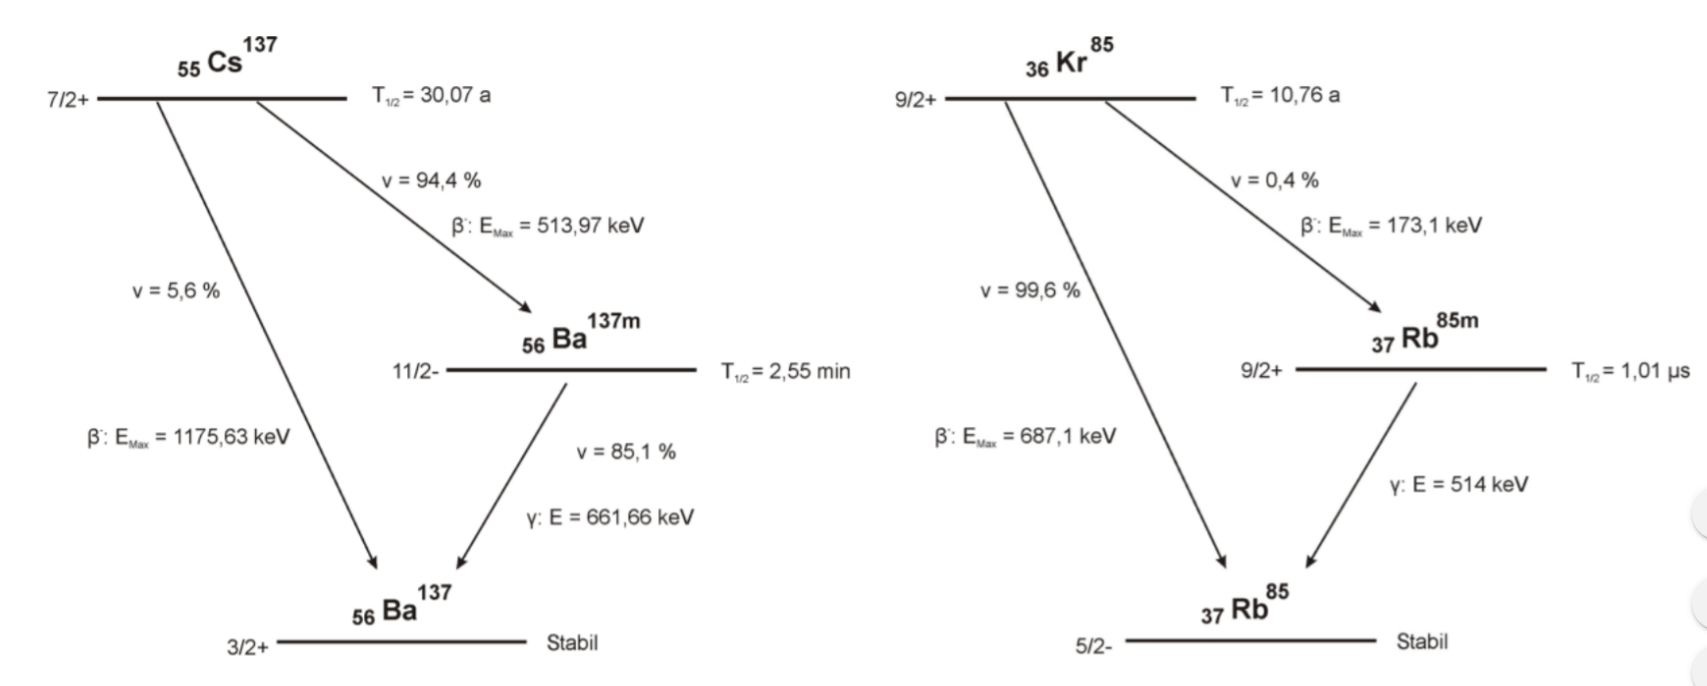
\includegraphics[width=\textwidth]{zerfallsschemata}
\caption{Vereinfachte Zerfallsschemata von $^{137}_{\ 55}$Cs und $^{85}_{36}$Kr, entnommen aus \cite{Anleitung}.}
\end{figure} \\\\
Dabei ist bei dem Schema von $^{137}_{\ 55}$Cs zu beachten, dass der Übergang von $^{137\mathrm{m}}_{\ \ \ 56}$Ba also angeregtem Barium, in den Grundzustand
$^{137}_{\ 56}$Ba auf zwei Arten geschehen kann:
\begin{itemize}
\item durch Emission eine $\gamma$-Quants
\item durch Abregung mittels Konversionselektronen
\end{itemize}
Letzteres kann erfolgen, wenn sich die Wellenfunktionen von Kern und Hüllenelektron überlappen. Es gibt dann einen Energieübertrag vom Kern auf das Elektron. Ist der Übertrag mindestend so groß wie die Bindungsenergie, kann das Elektron herausgelöst werden. Demzufolge ist die Energie der Konversionselektronen:
\begin{align*}
E_{\mathrm{IC}} = E_{\gamma} - E_B.
\end{align*}
$E_{\gamma}$ ist die Energie des angeregten Kerns und $E_\mathrm{B}$ die Bindungsenergie des Elektrons.
\\\\
Zur Beschreibung der Rate dieses Prozesses wird der Konversionskoeffizient $\alpha$ eingeführt:
\begin{align*}
\alpha = \frac{N_{\mathrm{IC}}}{N_{\gamma}} = \frac{N_{\mathrm{IC}}}{N_{\text{ges}} - N_{\mathrm{IC}}}.
\end{align*}
$N_{\mathrm{IC}}$ ist die Anzahl der Abregungen über innere Konversion(IC), $N_{\gamma}$ die Zahl der $\gamma$-Umwandlungen und $N_{\text{ges}}$ die Gesamtzahl der gemessenen Umwandlungen über $^{137\mathrm{m}}_{\ \ \ 56}$Ba. $\alpha$ besitzt dabei folgende Abhängigkeiten:
\begin{itemize}
\item sinkt stark mit steigendem $E_{\gamma}$
\item steigt stark mit Multipolordnung $L$
\item steigt mit Kernladungszahl $Z$
\item sinkt mit Hauptquantenzahl $n$
\end{itemize}

\subsection{Fermi-Plot}
Da im gemessenen $\beta$-Spektrum die Endpunkte durch die Konversionspeaks dominiert werden, ist die Bestimmung der Maximalenergie der $\beta$-Strahlung schwierig. Deshalb wird zu einem Fermi-Plot übergegangen. Dies ist eine linearisierte Darstellung, welche folgende Form hat:
\begin{align*}
\sqrt{\frac{N(E)}{p \cdot W \cdot F(Z,E)}} = c \cdot (E_0-E).
\end{align*}
Dabei ist $c$ die Proportionalitätskonstante, $p$ der Impuls, $W$ die Gesamtenergie, $N(E)$ die Zählungen im jeweiligen Energieintervall, $E_0$ die gesuchte Maximalenergie und $F(Z,E)$ die Fermi-Funktion, welche für $^{137}_{\ 55}$Cs den Wert $6$ und für $^{85}_{36}$Kr den Wert $5$ hat.

\subsection{Energieverlust beim Durchdringen von Materie}
Es gibt zwei Modelle, die den Energieverlust von Teilchen beim Durchdringen von Materie gut beschreiben: Die Bethe-Bloch Gleichung und das Landau-Modell. Das Modell von Landau beschreibt idR. den maximalen Energieverlust gut, während die Bethe-Bloch-Formel vor allem zur Berechnung des mittleren Energieverlustes geeignet ist. 
Der Energieverlust der Konversionslektronen soll deshalb mit beiden Ansätzen verglichen werden.

\subsubsection{Bethe-Bloch-Gleichung}
Die Bethe-Bloch-Gleichung für relativistische Teilchen lautet:
\begin{align*}
- \frac{1}{\rho} \left \langle \frac{\mathrm{d}E}{\mathrm{d} x} \right \rangle=
z^2 \frac{K}{2} \frac{Z}{A} \frac{1}{\beta^2} \left[ \ln \left(\frac{\tau^2(\tau+2)}{2(I/m_{\mathrm{e}}^2}\right)+F(\tau)- \delta(\beta \gamma)\right].
\end{align*}
Dabei sind die auftretenden Größen:
\begin{itemize}
\item $\beta=\frac{v}{c}$
\item $\tau = \gamma -1$
\item $\rho$ Dichte des Materials
\item $Z$ Kernladungszahl des Materials
\item $A$ Massenzahl des Materials
\item $m_{\mathrm{e}}$ Ruhemasse des Elektrons
\item $z$ Ladung der einfallenden Teilchen
\item $I$ Anregungsenergie: $I = 150$\,eV für Aluminium
\item $F(\tau) = 1- \beta^2+\frac{\frac{\tau^2}{8}- \ln 2(2\tau+1)}{(\tau+1)^2}$ (berücksichtigt Ununterscheidbarkeit der Teilchen)
\item $K = 4 \pi N_{\mathrm{A}} r_{\mathrm{e}}^2 m_\mathrm{e} \approx 0.3071$\, MeV $\text{mol}^{-1}$ $\text{cm}^2$ (Konstante)
\item $N_A = 6.022 \cdot 10^{23}$\,$\text{mol}^{-1}$ (Avogadro-Konstante)
\item $r_\mathrm{e} = 2.818$\,fm (klassischer Elektronenradius)
\item $\delta(\beta \gamma)$ Polarisationsverlust (wird vernachlässigt)
\end{itemize}

\subsubsection{Landau-Modell}
Die Abschätzung des Energieverlustes im Landau-Modell hat folgende Form:
\begin{align*}
\Delta E =z^2 \frac{K}{2} \frac{Z}{A} \frac{\rho}{\beta^2}x \left[ \ln \left(\frac{KZm_{\mathrm{e}}\rho}{2I^2(1-\beta^2)A}x\right)- \beta^2- \delta(\beta \gamma)\right].
\end{align*}
Es wird erwartet, dass die experimentellen Werte zwischen Bethe-Bloch und Landau liegen.

\subsection{Detektion von $\beta$-Strahlung}
Zur Detektion der $\beta$-Strahlung wird ein Silizium-Halbleiterdetektor verwendet. Es handelt sich um eine Kombination eines p- und eines n-dotierten Kontaktes aus halbleitendem Material, das in Sperrrichtung geschalten wird. An der Kontaktstelle der beiden Leiter bildet sich ein pn-Übergang, in dem Elektronen und Löcher rekombinieren. Dadurch entsteht eine Verarmungszone, die weitgehend frei von Ladungsträgern ist. Ionisierende Strahlung kann in dieser Verarmungszone Elektronen-Loch-Paare erzeugen, welche über die angelegte Spannung ($60$\,V) sofort abgesaugt werden. Es ergibt sich ein elektrisches Signal,welches man verstärken und anschließend einem Pulshöhenanalysator zuführen kann. Damit ist es möglich, einzelne auftreffende Elektronen, \(\gamma\)-Quanten sowie \(\alpha\)-Teilchen zu detektieren und zu zählen. Der Computer generiert daraus ein Übersichtsspektrum, das jedem Kanal eine Trefferhäufigkeit zuordnet. Durch eine Energiekalibrierung mit Strahlung bekannter Energie können die Häufigkeitsverteilungen dann in ein Energiespektrum umgerechnet werden, welches sich auswerten lässt. \\\\
Zu beachten ist, dass der Detektor prinzipiell auf jede Art von ionisierender Strahlung anspricht. Das ist nicht ganz unproblematisch, weil die verwendeten Nuklide neben dem Betaspektrum noch ein charakteristisches \(\gamma\)-Spektrum emitieren. Hier kann man sich zunutze machen, dass man Elektronen durch eine dünne Schicht aus Metall praktisch vollständig abschirmen kann; hochenergetische Photonen der \(\gamma\)-Strahlung jedoch nicht. Daher wird einmal das gesamte Spektrum aufgenommen und anschließend das Spektrum mit einer Aluminiumplatte als Hindernis um die Elektronen zu stoppen. Mit dieser zweiten Messung erhält man das reine \(\gamma\)-Untergrundspektrum, welches sich dann nachträglich aus dem Gesamtspektrum entfernen lässt. Auf diese Weise kann man das reine \(\beta\)-Spektrum untersuchen.

\newpage
\section{Durchführung}
\begin{itemize}
\item Aufnahme des $\beta$-Spektrums für $^{137}_{\ 55}$Cs
\item Abdecken der $^{137}_{\ 55}$Cs-Quelle mit Aluminium-Platte und Aufnahme des Untergrundspektrums
\item Abdecken der $^{137}_{\ 55}$Cs-Quelle mit Papier (1,2,3,4 Blätter) und Aufnahme des Spektrums
\item Abdecken der $^{137}_{\ 55}$Cs-Quelle mit Aluminium-Folie (3,6,9,12 Folien) und Aufnahme des Spektrums
\item Aufnahme des $\beta$-Spektrums für $^{85}_{36}$Kr
\item Bedecken der $^{85}_{36}$Kr-Quelle mit Aluminium-Platte und Aufnahme des Untergrundspektrums
\item Bedecken der $^{85}_{36}$Kr-Quelle mit Papier (1,2,3,4 Blätter) und Aufnahme des Spektrums
\item Bedecken der $^{85}_{36}$Kr-Quelle mit Aluminium-Folie (3,6,9,12 Folien) und Aufnahme des Spektrums
\item Messung der Röntgenlinien von Blei durch Anregung einer dünnen Bleifolie mit der \(\gamma\)-Strahlung der $^{85}_{36}$Kr-Quelle
\item Aufnahme des Spektrums einer \(^{241}_{\ 95}\)Am-Quelle für einen zusätzlichen Messpunkt zur Kalibrierung
\end{itemize}

\newpage
\section{Auswertung}
Grundlage für die gesamte Auswertung ist die Energiekalibrierung. Hierfür wurden insgesamt fünf bekannte Energiewerte verwendet, die im folgenden kurz vorgestellt werden. Nach dem Abdecken der \(^{137}_{\ 55}\)Cs-Quelle mit der Aluminiumplatte ergab sich der \(\gamma\)-Untergrund, der in Abb.5 dargestellt ist.\\
\begin{figure}[h!]\centering
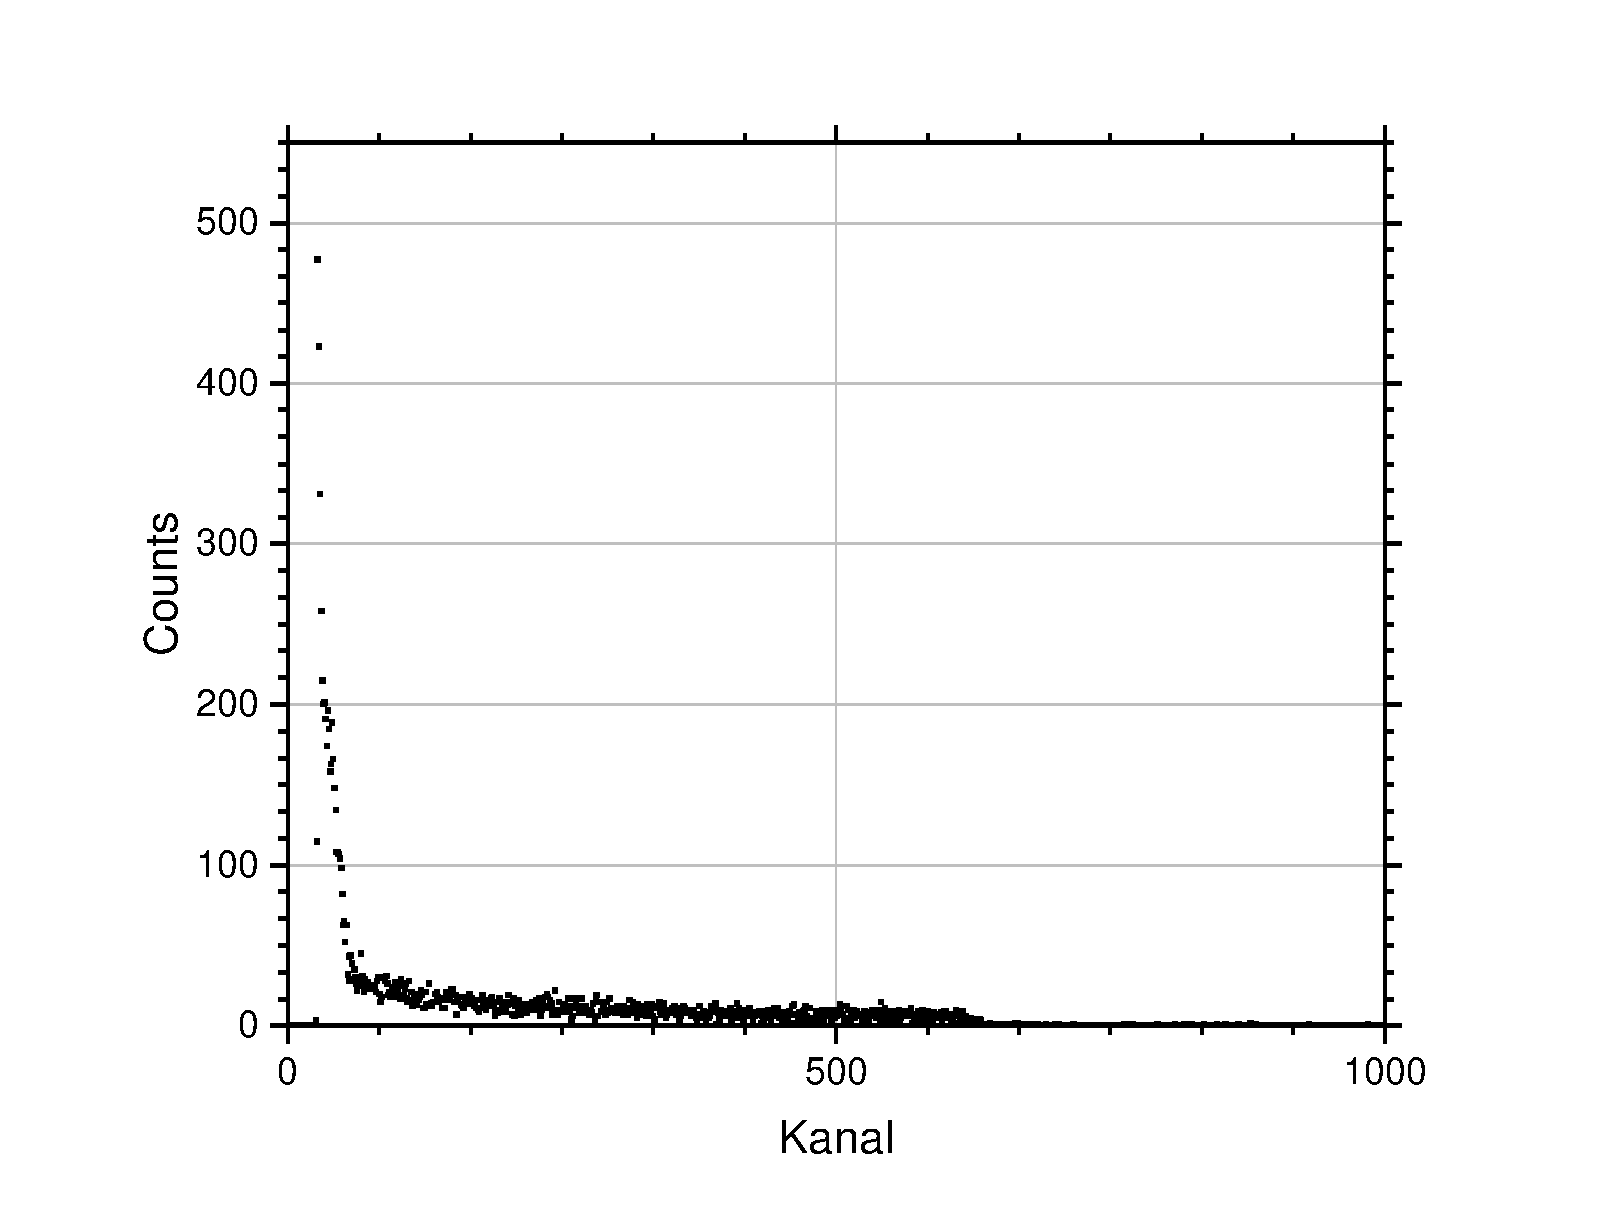
\includegraphics[width=\textwidth]{/home/tom/BE/Plots/CS_AL_plot.pdf}
\label{Cs-Untergrund_Kanal}
\caption{\(\gamma\)-Untergrund von \(^{137}_{\ 55}\)Cs, dargestellt als Ereignisse über Kanälen.}
\end{figure}\\
Interessant für die Kalibrierung ist die Compton-Kante. Um diese besser sichtbar zu machen, wurde der \(\gamma\)-Untergrund auf den relevanten Bereich eingeschränkt (Abb.6). 
\newpage
\begin{figure}[h!]\centering
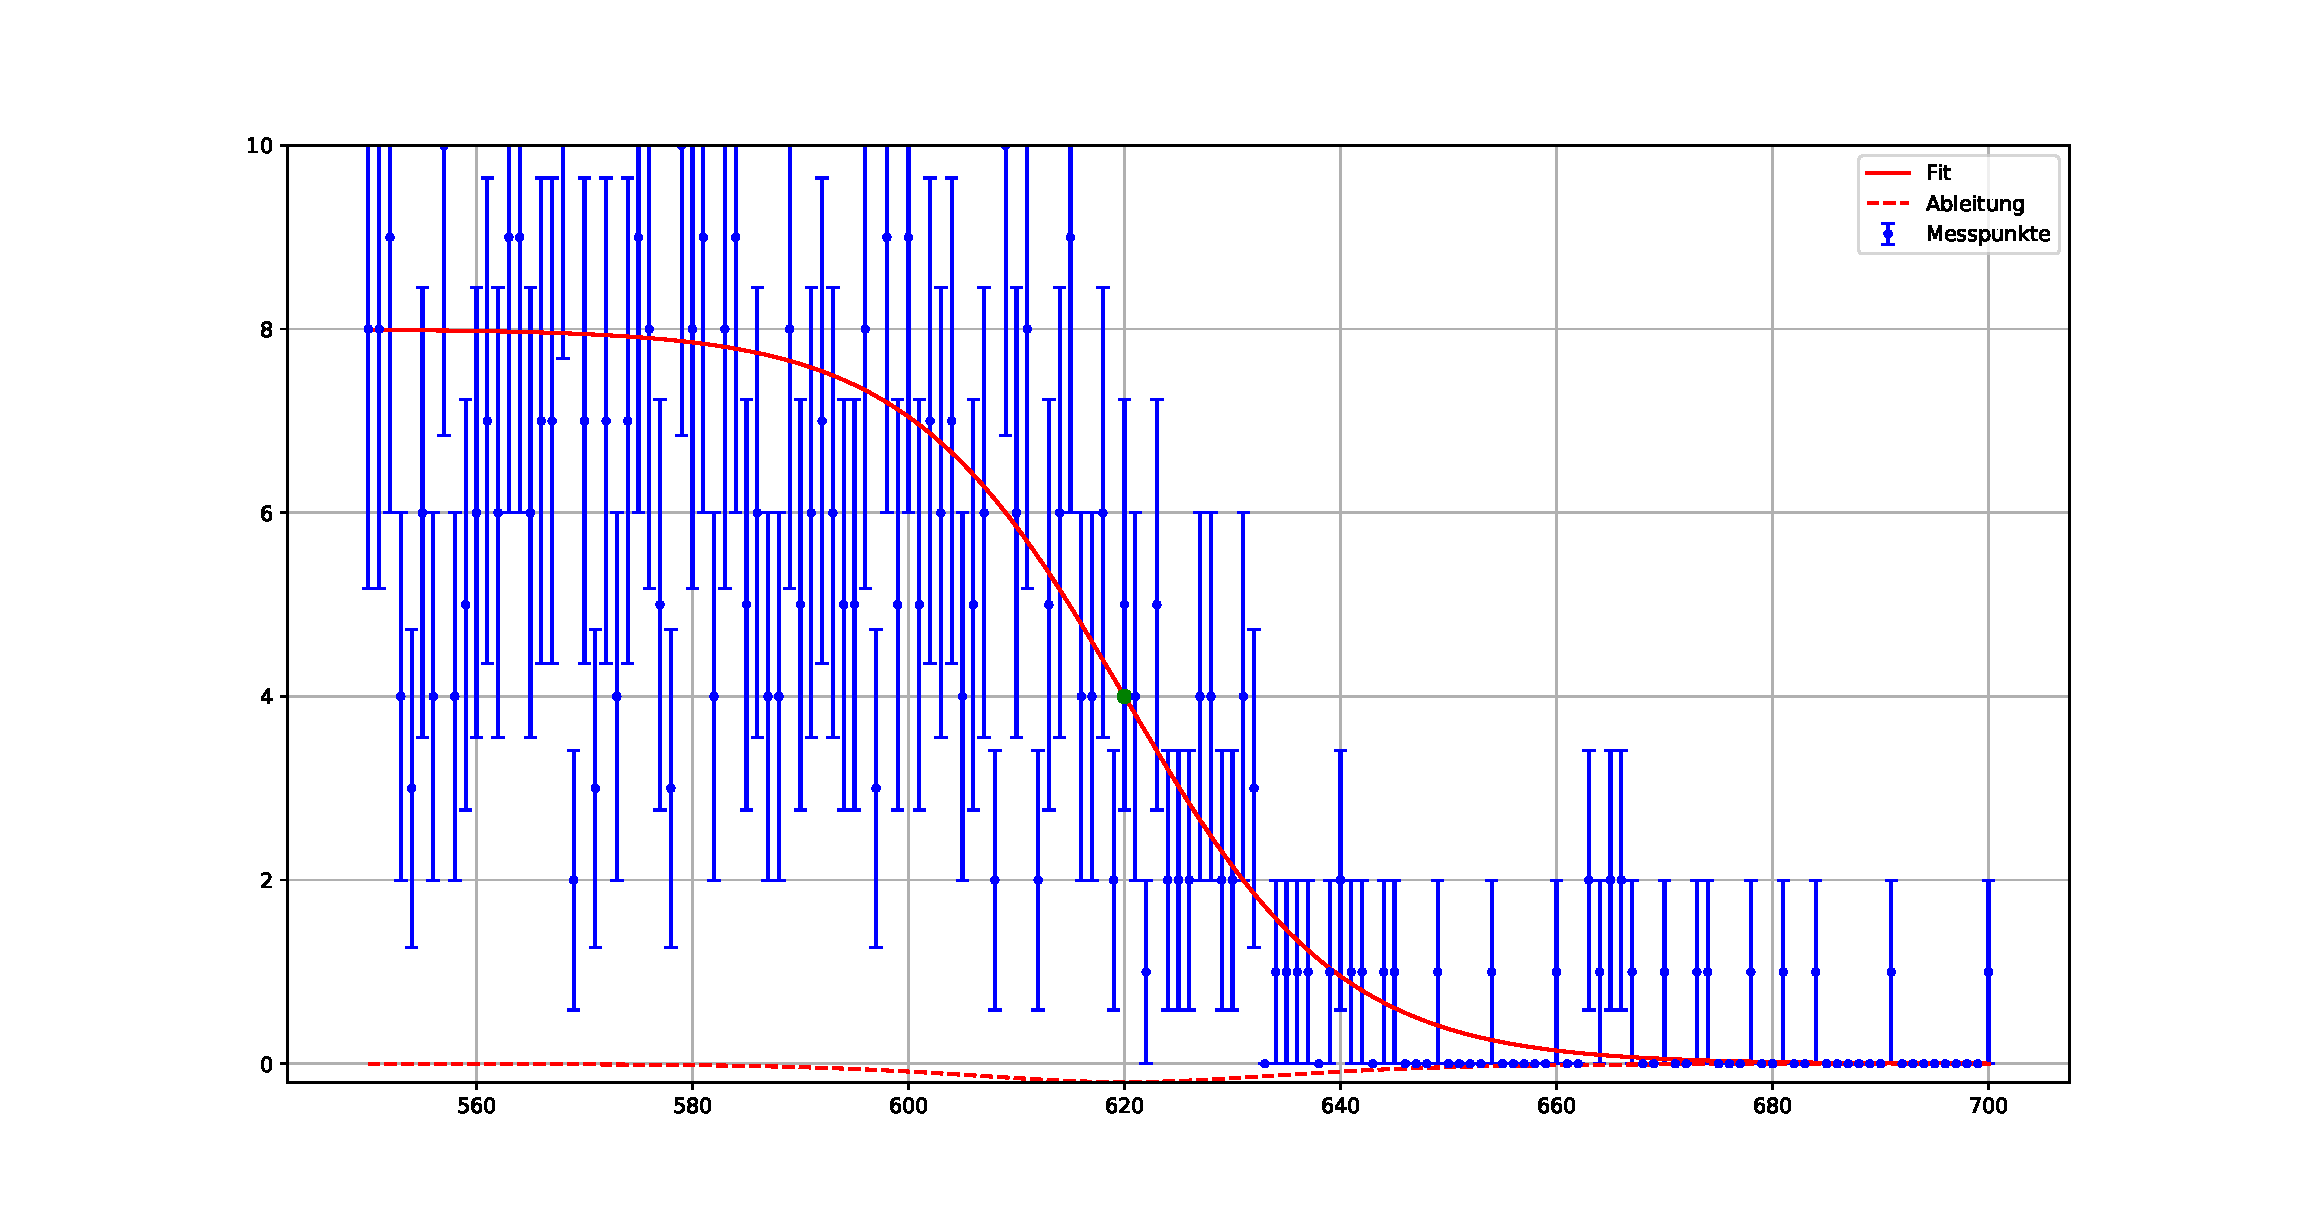
\includegraphics[width=\textwidth]{/home/tom/BE/Plots/Comptonkante.pdf}
\label{Compton-Kante}
\caption{Darstellung der Comptonkante von \(^{137}_{\ 55}\)Cs, dargestellt als Ereignisse über Kanälen.}
\end{figure}
Aufgrund der recht großen Unsicherheit ist die Bestimmung der Kanallage durch Fit mit der Methode der kleinsten Quadrate nicht möglich gewesen, da die Rechnung nicht konvergent war. Deshalb wurde nach Augenmaß eine Kurve möglichst gut angepasst und die Unsicherheit geschätzt. Als Funktion wurde eine Fermi-Verteilung verwendet:
\begin{align*}
y(x) = \frac{a}{1 + \exp\left(\frac{x-b}{c}\right)} \quad\text{mit}\quad a = 8,\, b= 620,\, c= 10.
\end{align*}
Interessant für die Auswertung ist ohnehin nur der Parameter \(b\), für diesen wurde der Wert samt Unsicherheit zu \(b=(620\pm 10)\) geschätzt. Dieser Wert entspricht der Kanallage der Compton-Kante. Die beim Übergang von \(^{137\mathrm{m}}_{\ \ \ 56}\)Ba in den Grundzustand emittierten Photonen haben eine Energie von \(E_{\gamma} = 661.66\,\mathrm{keV}\), wie man aus dem Zerfallsschema in Abb. 3 entnehmen kann. An der Comptonkante kommt es zum maximalen Energieübertrag auf Elektronen. Der maximale Energieübertrag kann nach der Compton'schen Streuformel berechnet werden, da der maximale Energieübertrag bei Rückstreuung mit \(\vartheta=\pi\) stattfindet:
\begin{align*}
E_{\mathrm{e}}^{\mathrm{max}} = \left.\frac{E_{\gamma}^2(1-\cos\vartheta)}{m_{\mathrm{e}} + E_{\gamma}(1-\cos\vartheta)}\right|_{\vartheta=\pi} = \frac{2E_{\gamma}^2}{m_{\mathrm{e}} + 2E_{\gamma}} = 477.34\,\mathrm{keV}.
\end{align*}
Wir erhalten dementsprechend eine Zuordnung der Energie von \(E=477.34\,\mathrm{keV}\) zum Kanal \((620\pm 10)\), womit ein Punkt der Kalibrierung bestimmt ist. \\\\
Zwei weitere Punkte ergaben sich aus den Konversionspeaks. Dazu wurden zunächst die detektierten Ereignisse für \(^{137}_{\ 55}\)Cs dargestellt (Abb. 7) und anschließend der Bereich mit den Konversionsübergängen herausgesucht (Abb. 8). \\\\
\begin{minipage}{0.5\textwidth}%\flushleft
\begin{flushleft}
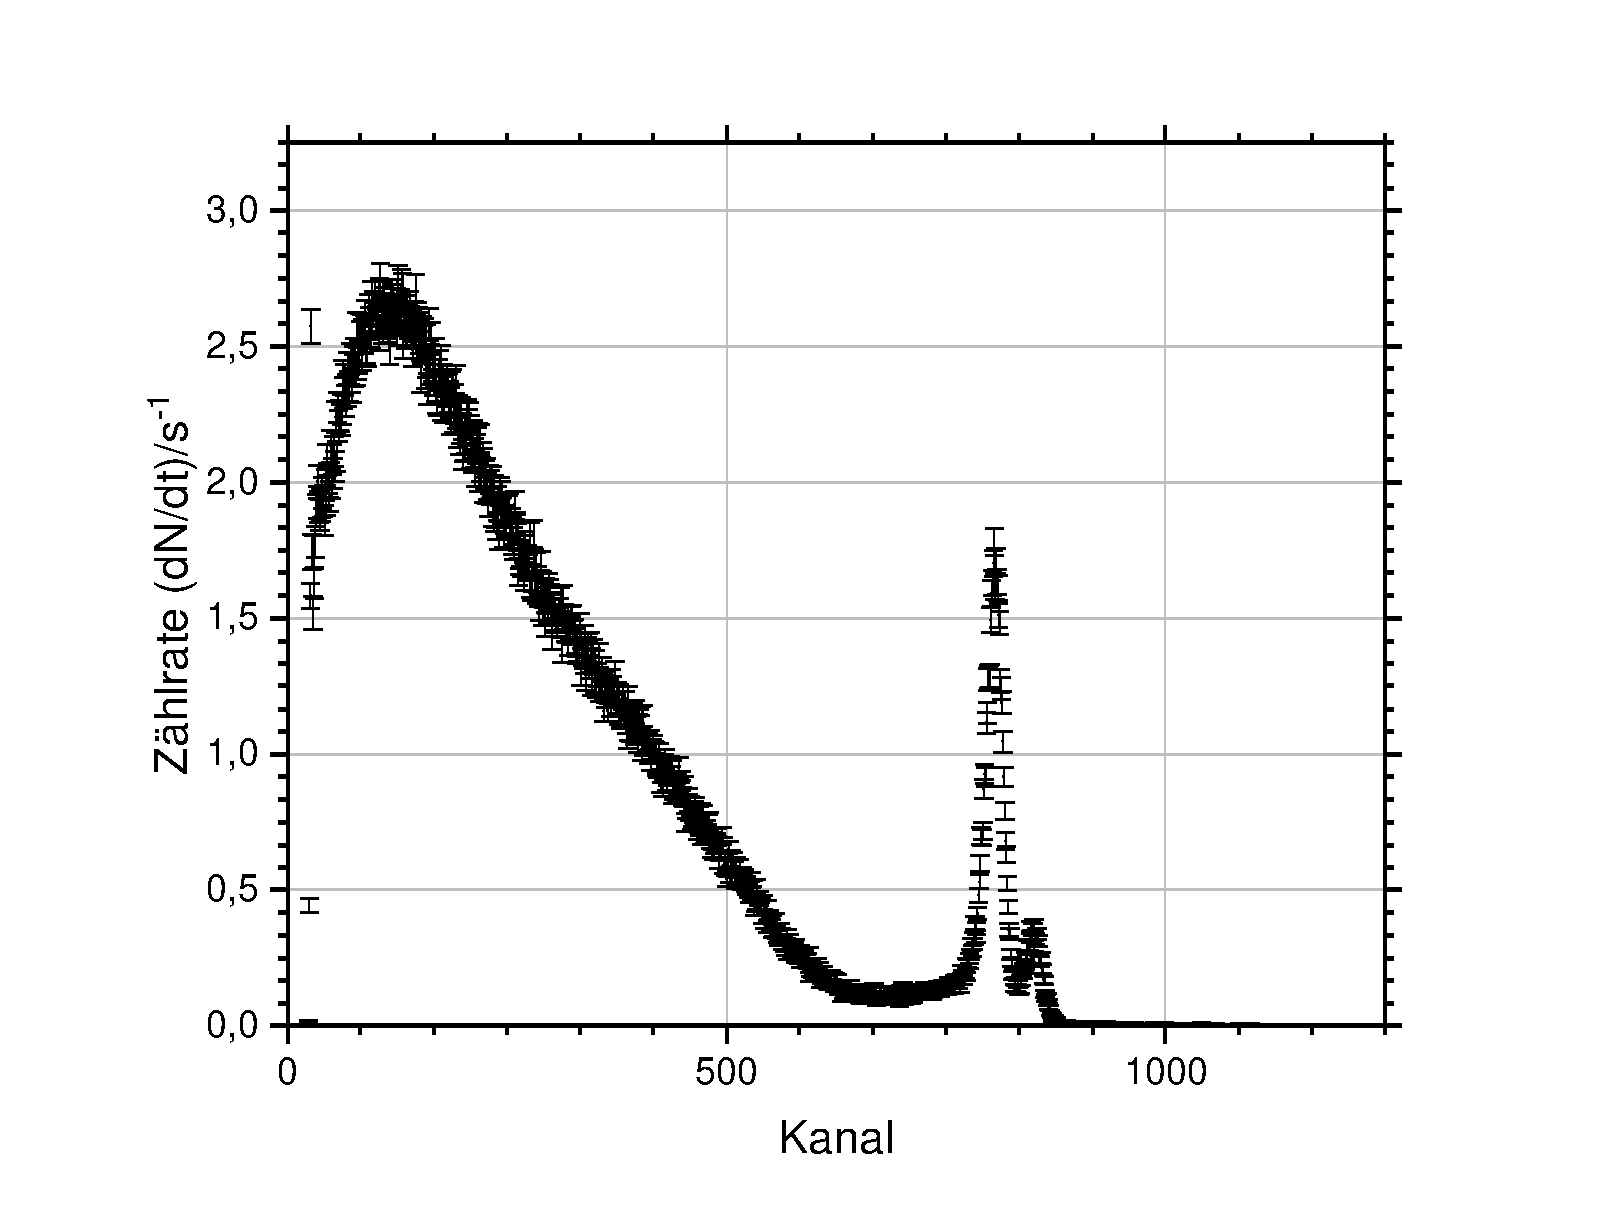
\includegraphics[width=\textwidth]{/home/tom/BE/Plots/CS_ohneUG_plot.pdf}
\captionof{figure}{Gesamtspektrum von \(^{137}_{\ 55}\)Cs.}
\end{flushleft}
\end{minipage}
%\begin{minipage}{0.1\textwidth}\centering
%\[\ \ \]
%\end{minipage}
\begin{minipage}{0.5\textwidth}%\flushleft
\begin{flushleft}
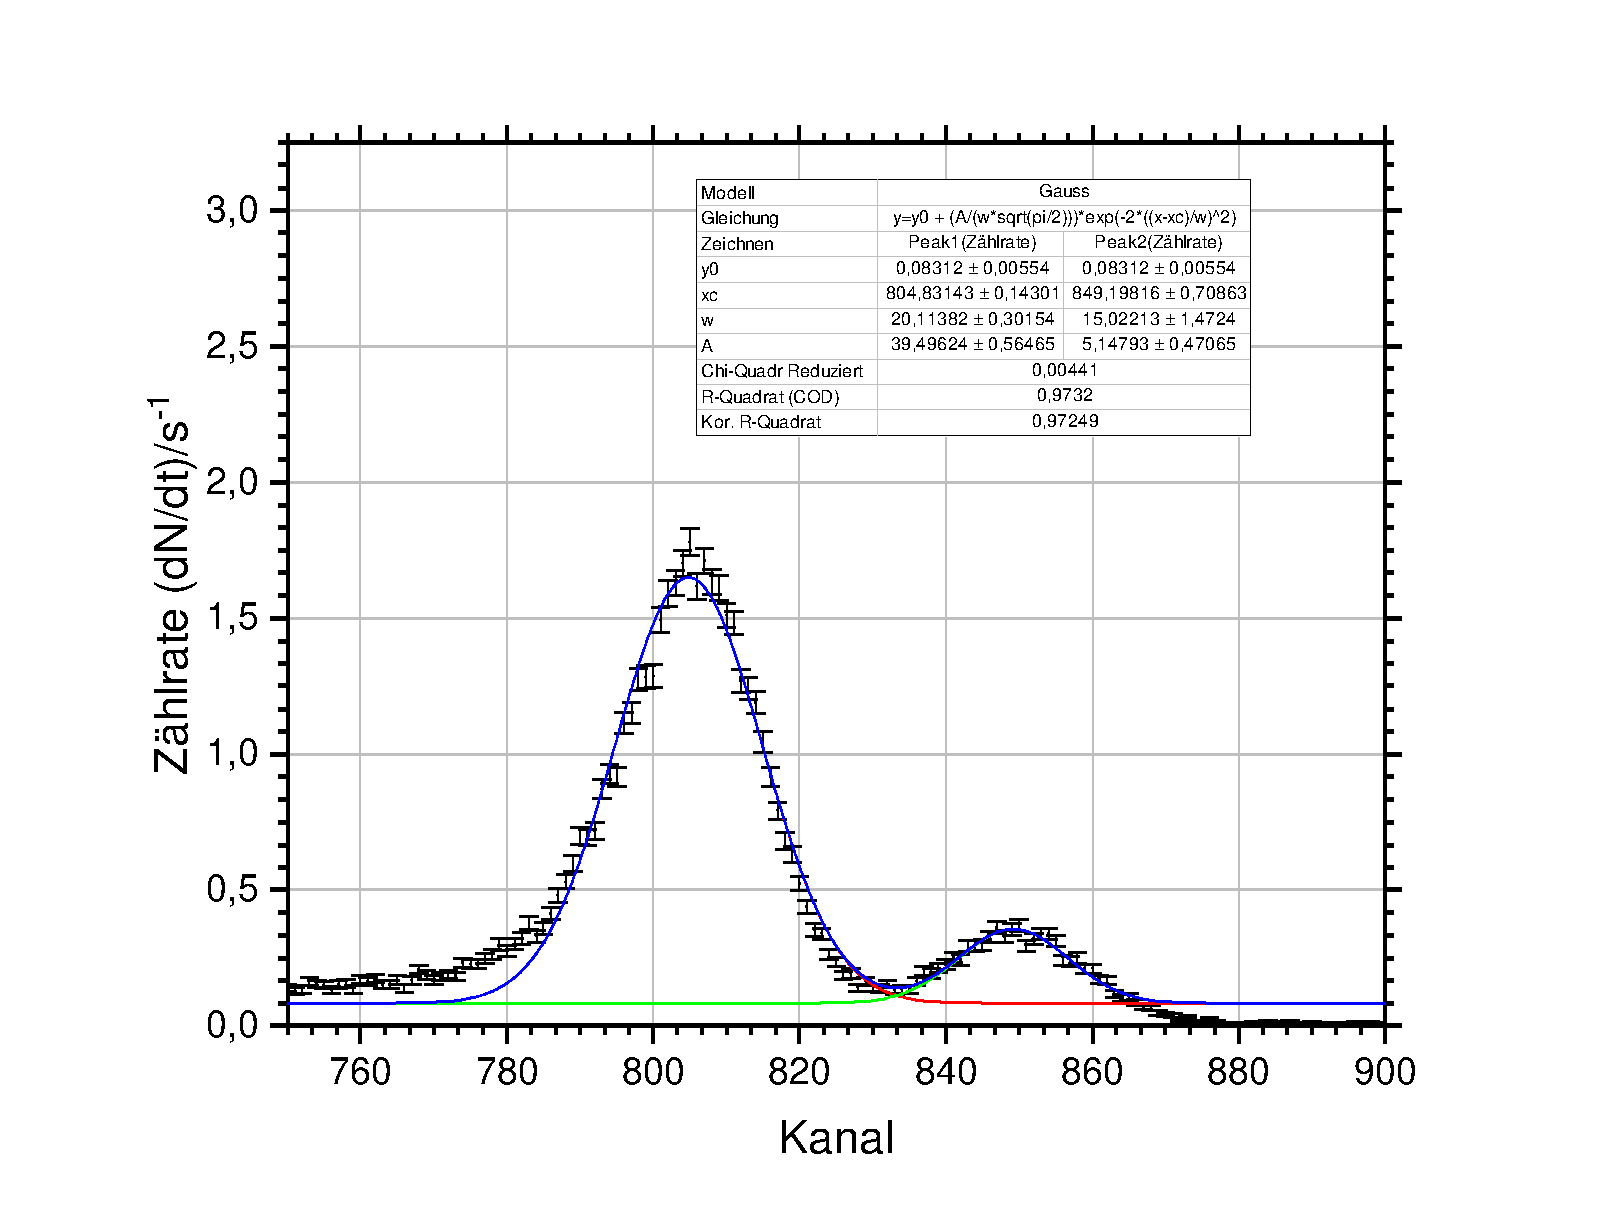
\includegraphics[width=\textwidth]{/home/tom/BE/Plots/CS_ohneUG_peaks.pdf}
\captionof{figure}{Innere Konversion von \(^{137}_{\ 55}\)Cs.}
\end{flushleft}
\end{minipage} \\\\
Die Konversionskoeffizienten beim Übergang von \(^{137\mathrm{m}}_{\ \ \ 36}\)Ba in den Grundzustand konnten aus \cite{Anleitung} entnommen werden. Sie betragen \(8.96\,\%\) für K-Elektronen und \(1.67\,\%\) für L-Elektronen. Da diese Koeffizienten der relativen Häufigkeit von Konversion gegenüber dem direkten \(\gamma\)-Übergang entsprechen, bilden sie ein Maß für die Intensität des entsprechenden Konversionspeaks. Dementsprechend ordnen wir den linken, wesentlich ausgeprägteren Peak den K-Elektronen und den linken, kleineren Peak den L-Elektronen zu. Das ist auch dahingehend konsistent, als dass der Überlapp der Kernwellenfunktion mit K-Elektronen signifikant höher ist mit L-Elektronen. Die Energie der Konversionselektronen ist jeweils die Energiedifferenz zwischen \(^{137\mathrm{m}}_{\ \ \ 36}\)Ba und dem Grundzustand von \(\Delta E = 661.66\,\mathrm{keV}\) abzüglich der Bindungsenergie der jeweiligen Schale. Die Bindungsenergien sind \(E_{\mathrm{Bind}}^{\mathrm{K}} = 37.441\,\mathrm{keV}\) bzw. \(E_{\mathrm{Bind}}^{\mathrm{L}} = 5.989\,\mathrm{keV}\). Die Energien der Konversionselektronen ergeben sich damit zu:
\begin{align*}
E_{\mathrm{IC}}^{\mathrm{K}} &= \Delta E - E_{\mathrm{Bind}}^{\mathrm{K}} = 624.219\,\mathrm{keV} \ \text{sowie}\\
E_{\mathrm{IC}}^{\mathrm{L}} &= \Delta E - E_{\mathrm{Bind}}^{\mathrm{L}} = 655.671\,\mathrm{keV}. \\
\end{align*}
Wie in Abb. 8 gezeigt, wurde die Kanallage durch Gaußfits bestimmt. Es ergaben sich Kanallagen von (805\(\pm\)0) für die K-Elektronen und (849\(\pm\)1) für die L-Elektronen.\\\\
Im Anschluss wird die \(\gamma\)-Strahlung der \(^{85}_{36}\)Kr-Quelle verwendet, um in einer dünnen Bleifolie charakteristische Röntgenübergänge anzuregen. Auch hier wurden die Zählraten über den Kanälen dargestellt, wie in Abb. 9 und Abb. 10  dargestellt. \\
\begin{minipage}{0.5\textwidth}\centering
%\begin{flushleft}
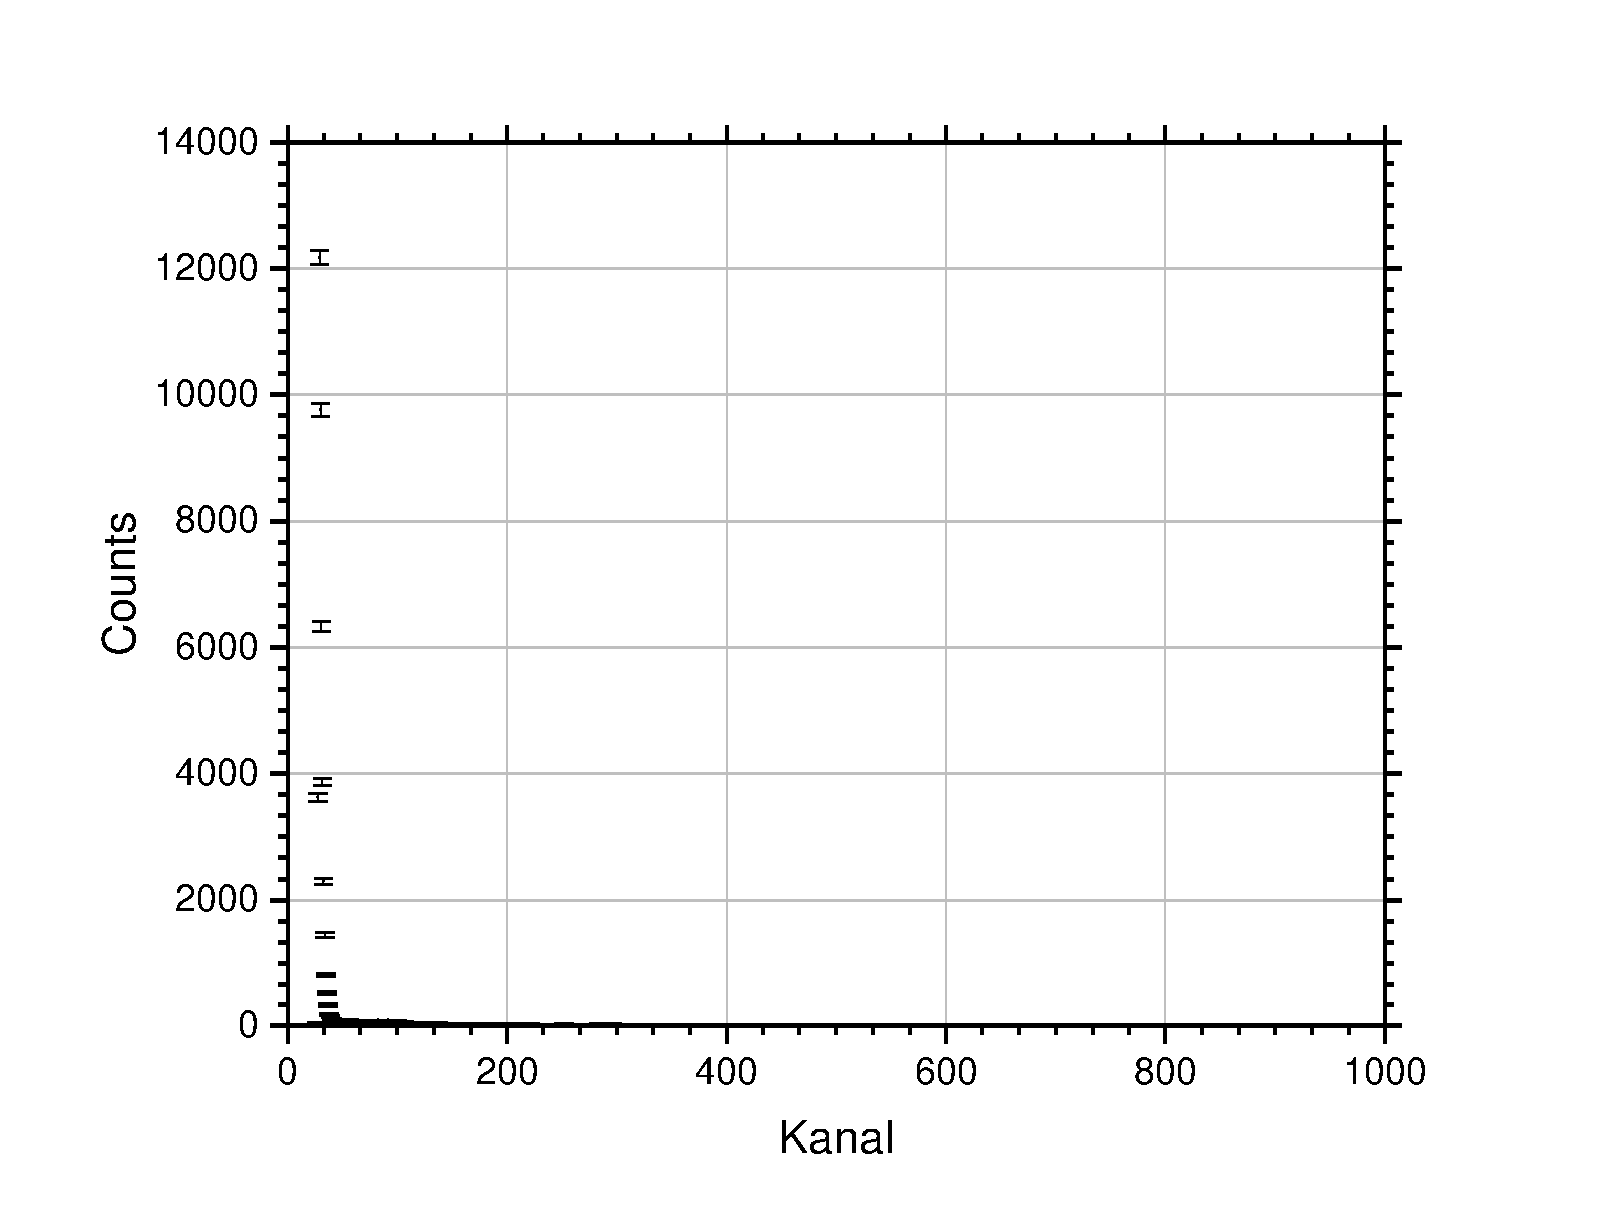
\includegraphics[width=\textwidth]{/home/tom/BE/Plots/Blei_plot.pdf}
\captionof{figure}{Röntgenspektrum von \(_{82}\)Pb.}
%\end{flushleft}
\end{minipage}
%\begin{minipage}{0.04\textwidth}\centering
%\[\ \ \]
%\end{minipage}
\begin{minipage}{0.5\textwidth}\centering
%\begin{flushright}
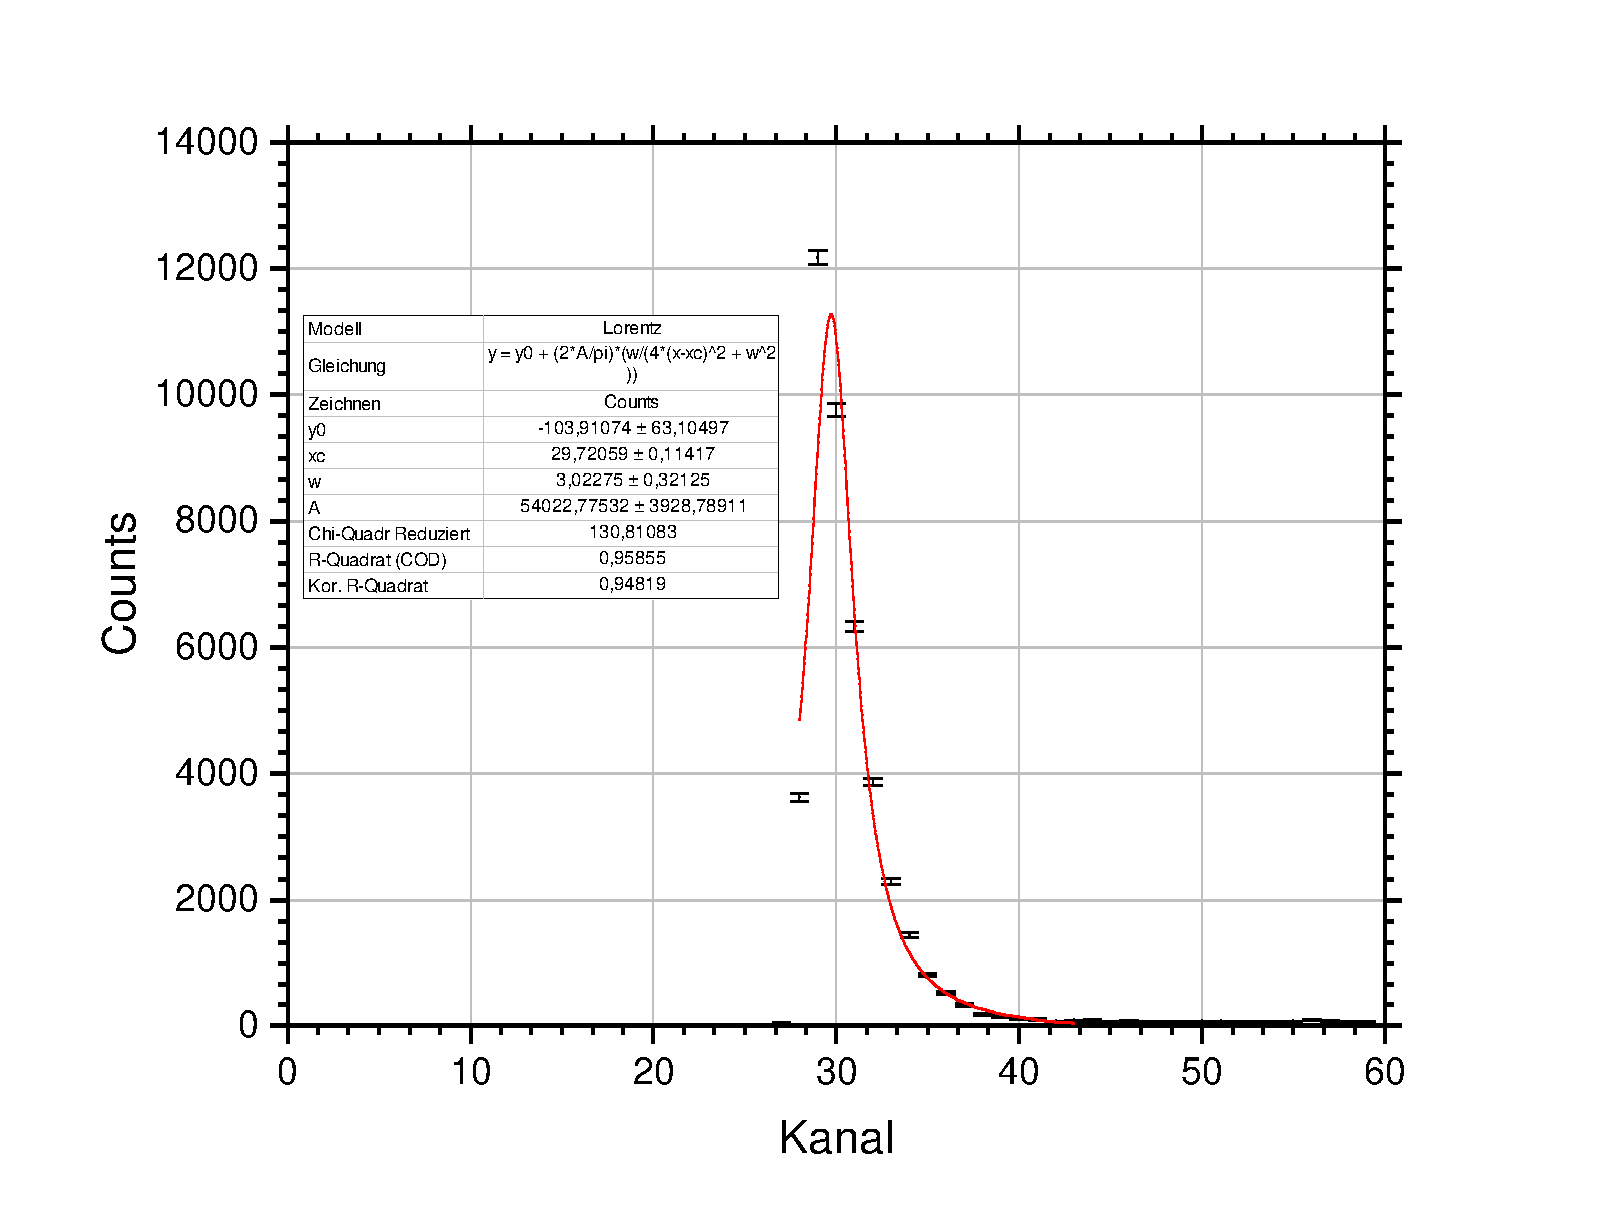
\includegraphics[width=\textwidth]{/home/tom/BE/Plots/Blei_peaks.pdf}
\captionof{figure}{Detailansicht des Peaks}
%\end{flushright}
\end{minipage} \\\\
Die Werte der charakteristischen Röntgenübergänge von Blei liegen tabelliert vor (entnommen aus \cite{Anleitung}).\\
\begin{table}[h!]\centering
\begin{tabular}{|c|c|c|}
\hline
Linie & \(E/\mathrm{keV}\) & \(I_{\mathrm{rel}}/\%\) \\\hline
\(\mathrm{K}_{\alpha 1}\) & \(74.969\) & \(46.80\) \\\hline
\(\mathrm{K}_{\alpha 2}\) & \(72.805\) & \(27.80\) \\\hline
\(\mathrm{K}_{\alpha 3}\) & \(72.144\) & \(0.043\) \\\hline
\end{tabular}
\caption{Charakteristische Röntgenübergänge von \(_{82}\)Pb.}
\end{table} \\\\
Der Übergang der \(\mathrm{K}_{\alpha 3}\)-Linie war aufgrund der geringen Intensität nicht zu beobachten. Die \(\mathrm{K}_{\alpha 1}\)- und die \(\mathrm{K}_{\alpha 2}\)-Linie liegen so eng beieinander, dass sie nicht getrennt aufgelöst werden können und wie ein Peak erscheinen. Deshalb wurde nur ein Fit durchgeführt und dieser dann der intensivsten Linie, d.h. dem \(\mathrm{K}_{\alpha 1}\)-Übergang zugeordnet. Aufgrund der Überlagerung der Linien führte ein Gaußfit hier nicht zur Konvergenz, weswegen eine Lorentzkurve verwendet wurde. Es ergab sich eine Kanallage von (\(30\pm 0\)). Es wurde hierbei darauf verzichtet, den Untergrund zu subtrahieren, weil die \(\gamma\)-Photonen nahezu vollständig in Röntgenstrahlung umgesetzt werden. \\\\
Abschließend wurde noch eine \(^{241}_{\ 95}\)Am-Quelle verwendet. Dieses Nuklid wandelt sich gemäß \(^{241}_{\ 95}\)Am \(\rightarrow\) \(^{237\mathrm{m}}_{\ \ \ 93}\)Np + \(^4_2\alpha\) unter \(\alpha\)-Zerfall in einen angeregten Neptuniumkern um, welcher dann unter \(\gamma\)-Emmision in den Grundzustand übergeht. Das zugehörige Spektrum zeigen Abb. 11 und Abb. 12:  \\
\begin{minipage}{0.5\textwidth}\centering
%\begin{flushleft}
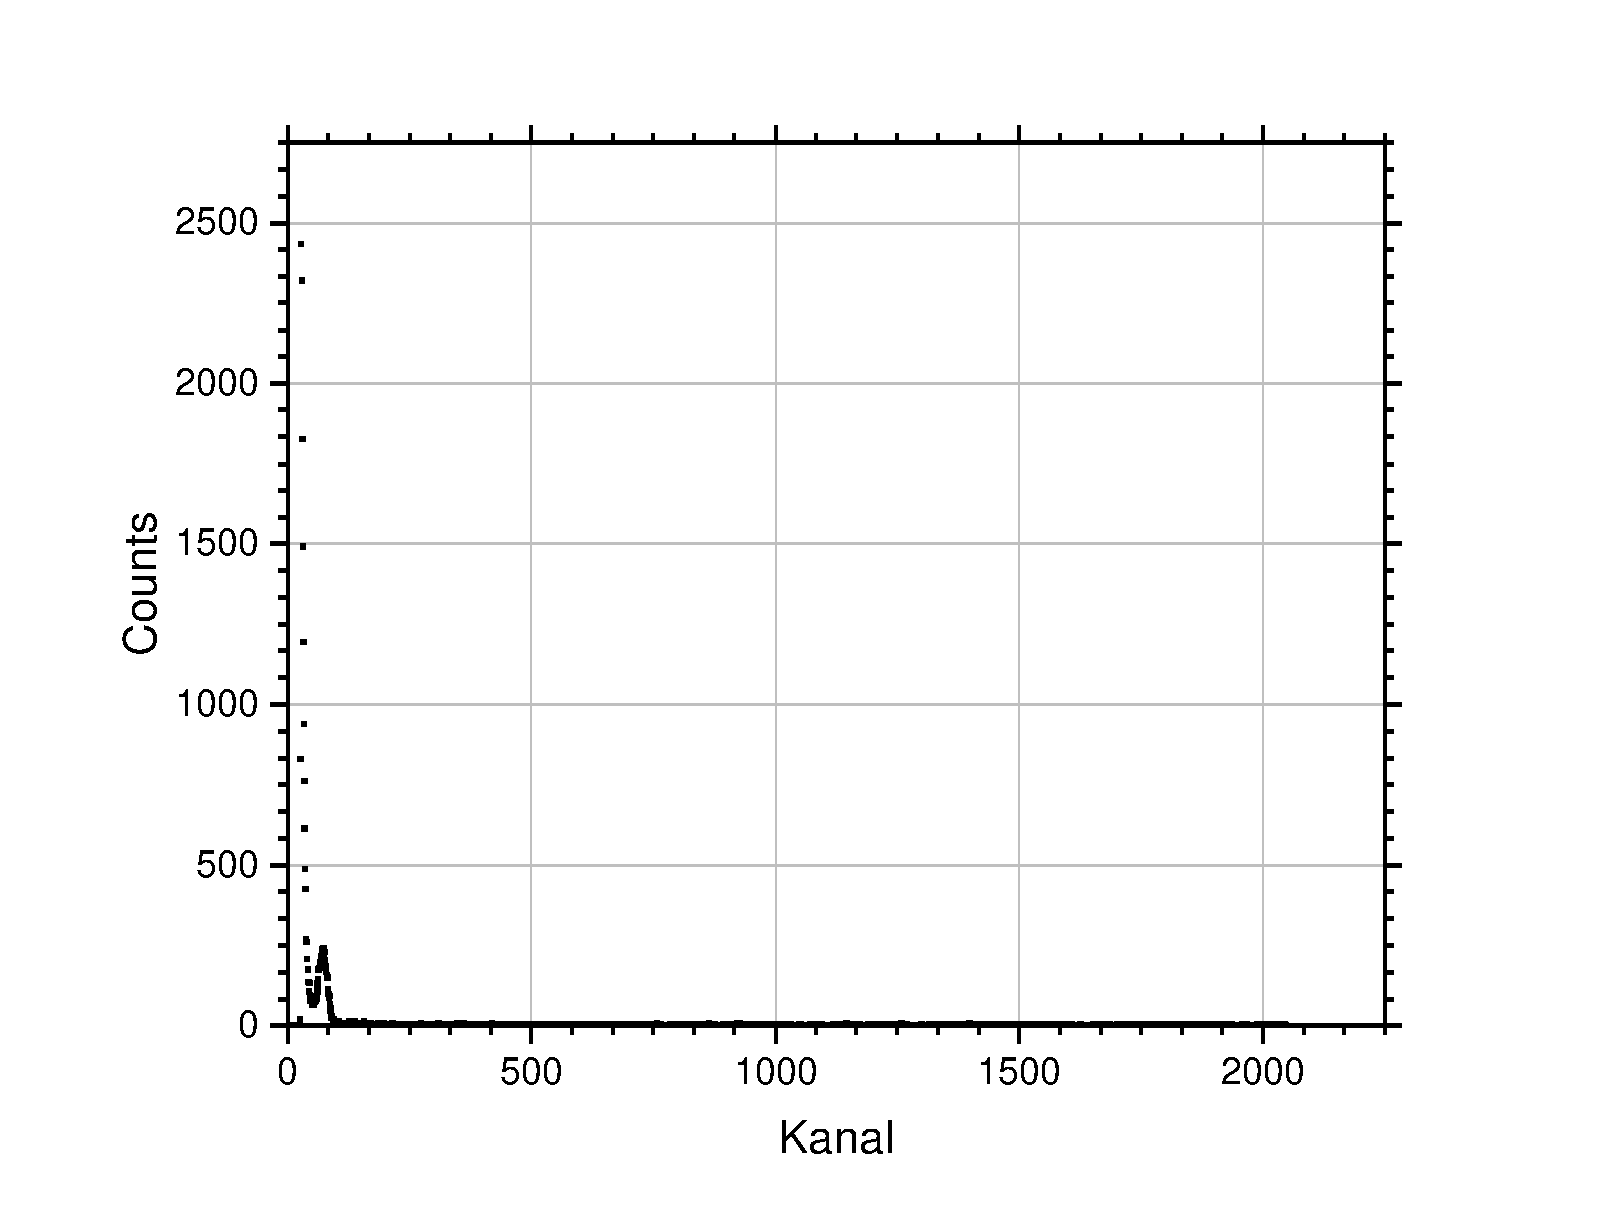
\includegraphics[width=\textwidth]{/home/tom/BE/Plots/AM_plot.pdf}
\captionof{figure}{Spektrum von \(^{241}_{\ 95}\)Am}
%\end{flushleft}
\end{minipage}
%\begin{minipage}{0.04\textwidth}\centering
%\[\ \ \]
%\end{minipage}
\begin{minipage}{0.5\textwidth}\centering
%\begin{flushright}
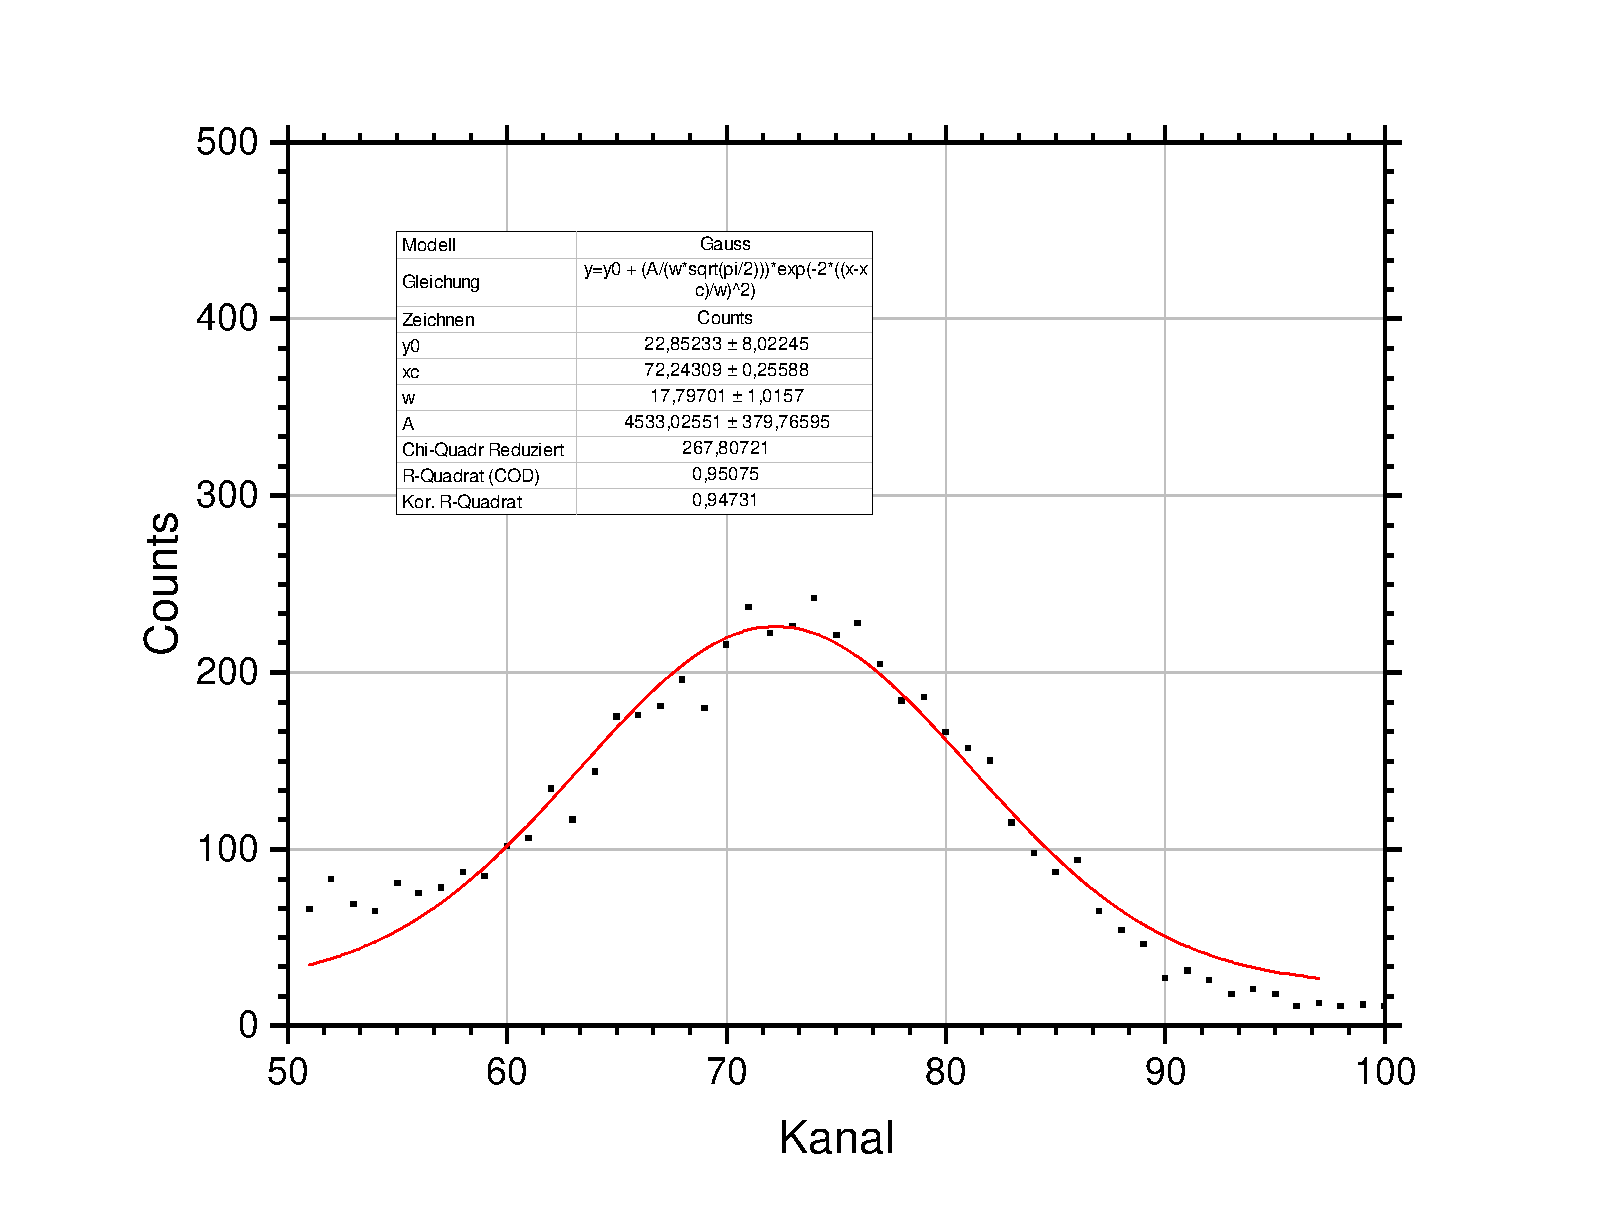
\includegraphics[width=\textwidth]{/home/tom/BE/Plots/AM_plot_peaks.pdf}
\captionof{figure}{Detailansicht des Peaks}
%\end{flushright}
\end{minipage} \\\\
Der \(\gamma\)-Übergang des Neptuniums ist ebenfalls bekannt und liegt bei \(39.5\,\mathrm{keV}\); dieser Wert wurde uns vom Betreuer mitgeteilt. Die Kanallage wurde mit einem Gaußfit zu (\(72\pm 0\)) bestimmt. Damit liegen fünf Messpunkte für die endgültige Kalibrierung vor, die in Tab. 2 zusammengestellt sind. \\
\begin{table}[h!]\centering
\begin{tabular}{|c|c|c|}
\hline
\((\mathrm{Kannal}\pm\Delta\mathrm{Kanal}\) & \((E/\mathrm{keV})\)& bestimmt mit \\\hline
\((620\pm 10)\) & \(477.34\) & Comptonkante des \(\gamma\)-Spektrums von \(^{137}_{\ 55}\mathrm{Cs}\) \\\hline
\((805\pm 0)\) & \(624.219\) & IC der K-Elektronen von \(^{137}_{\ 55}\mathrm{Cs}\) \\\hline
\((849\pm 1)\) & \(655.67\) & IC der L-Elektronen von \(^{137}_{\ 55}\mathrm{Cs}\) \\\hline
\((30\pm 0)\) & \(74.969\) & \(\mathrm{K}_{\alpha1}\)-Linie des Röntgenspektrums von \(_{82}\mathrm{Pb}\) \\\hline
\((72\pm 0)\) & \(39.5\) & \(^{241}_{\ 95}\mathrm{Am}\rightarrow ^{237\mathrm{m}}_{\ \ \ 93}\mathrm{Np} + ^4_2\alpha\rightarrow ^{237}_{\ 93}\mathrm{Np} + \gamma\), \(\gamma\)-Peak \\\hline
\end{tabular}
\caption{Verwendete Punkte zur Kalibrierung.}
\end{table} \\
\newpage
Damit kann eine Kalibrierung vorgenommen werden, wie in Abb. 13 dargestellt. \\
\begin{figure}[h!]\centering
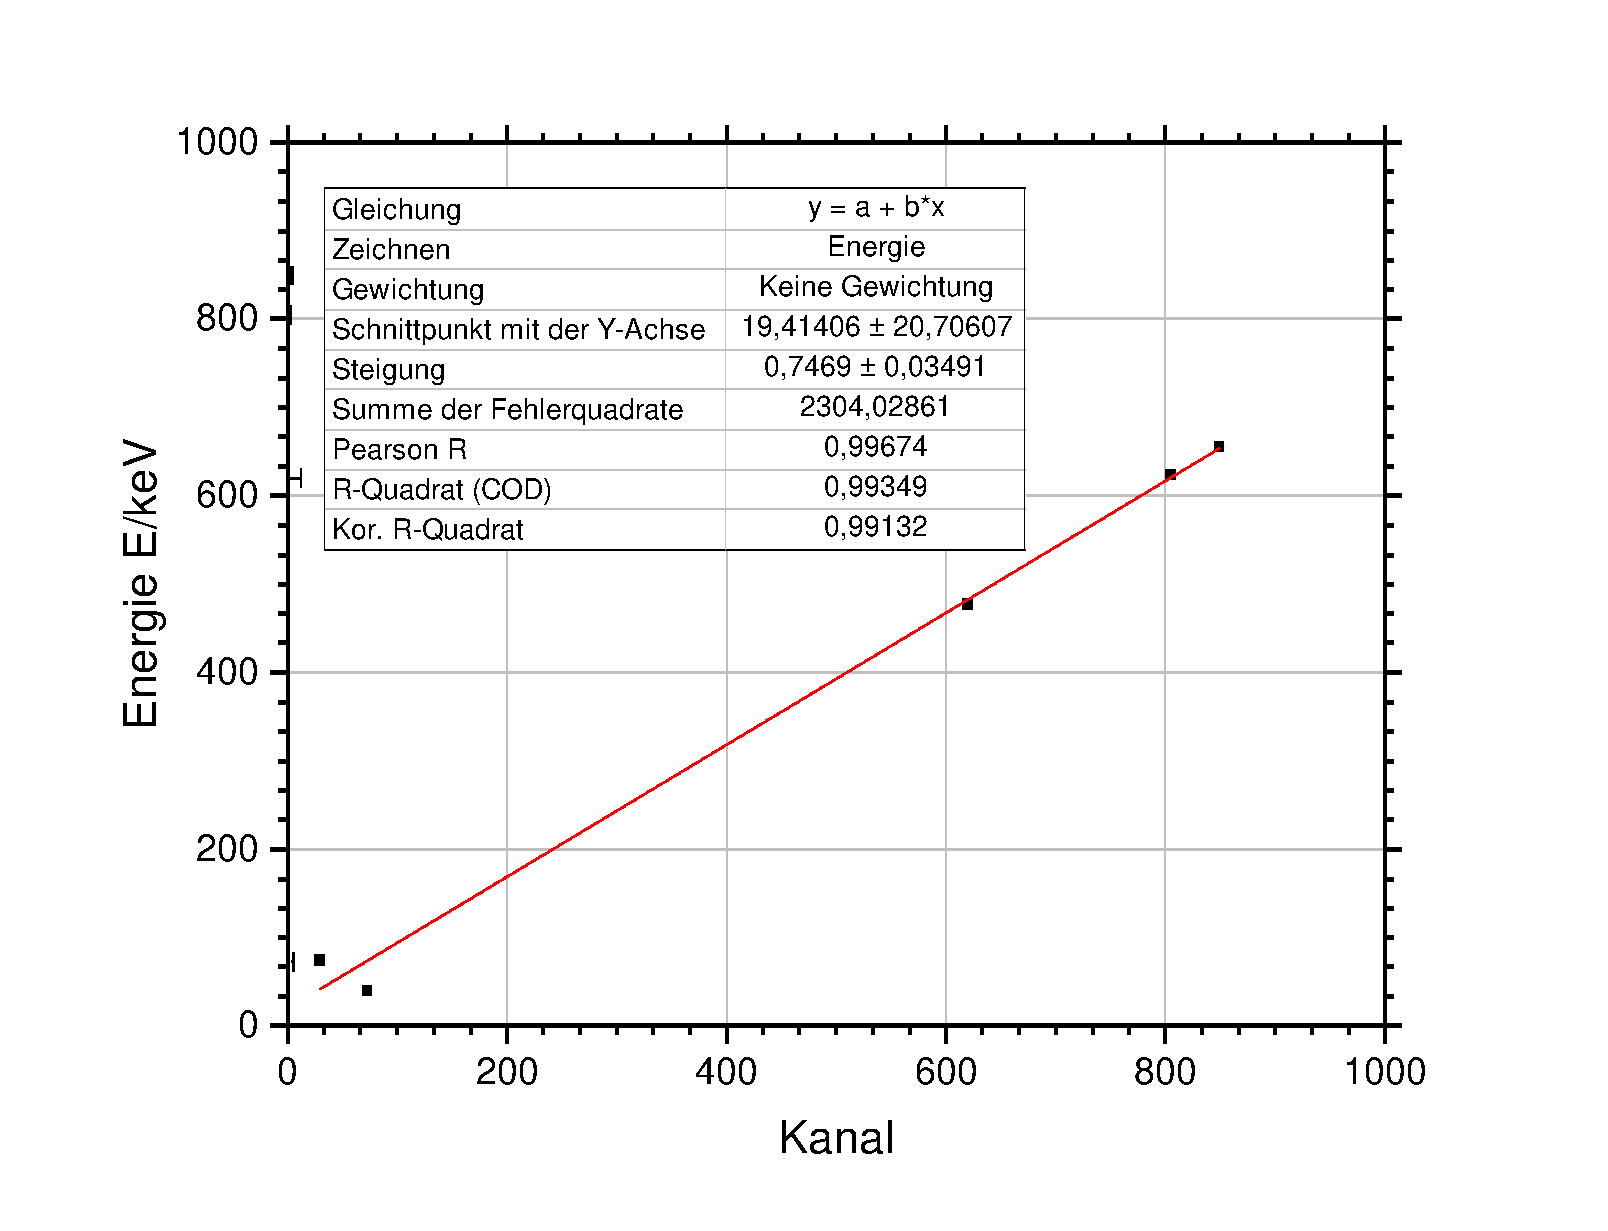
\includegraphics[width=\textwidth]{/home/tom/BE/Plots/Kalibrierung.pdf}
\caption{Erstellung einer Kalibriergeraden für die weitere Auswertung.}
\end{figure} \\\\
Es ist deutlich zu erkennen, dass die Kalibrierungspunkte in den unteren Kanälen etwas mehr von der Gerade abweichen, während die drei Punkte in den oberen Kanälen nahezu perfekt korreliert sind. Die beiden unteren Punkte gehören zur Röntgenlinie des Bleis bzw. zum Gammaübergang des Neptuniums, welches aus der Americium-Quelle entsteht. Die charakteristische Röntgenlinie hatte eine vergleichsweise hohe Unsicherheit, da sie sehr dicht neben einer weiteren Linie lag und wir diesen Unterschied nicht auflösen konnten. Die Gammalinie des Neptunium hatte eine ebenfalls größere Unsicherheit, weil sie im Spektrum verbreitert erschien (vgl. Abb. 12). Glücklicherweise lag die Röntgenlinie vom Blei oberhalb der Geraden und die Gammalinie vom Neptunium unterhalb, sodass sich beide Unsicherheiten bei der Regression in Summe größtenteils aufgehoben haben. Auf der Grundlage dieser Kalibrierung können nun sämtliche Messergebnisse über der Energie statt über Kanälen aufgetragen werden, sodass sich aussagekräftige Spektren ergeben.

\subsection{\(\gamma\)-Untergrund von \(^{137}_{\ 55}\mathrm{Cs}\) und \(^{85}_{36}\mathrm{Kr}\)}
Da beide hier untersuchten Nuklide sowohl \(\beta^-\)-Umwandlungen als auch \(\gamma\)-Übergänge aufweisen, muss zuerst das \(\gamma\)-Spektrum extrahiert werden. Hierzu wurden die Elektronen der \(\beta^-\)-Strahlung mit einer Aluminiumplatte ausgefiltert, sodass der Detektor nur die Photonen der \(\gamma\)-Strahlung detektierte. Zieht man die Zerfallsschemate aus Abb. 4 zu Rate, kann man die maximale Energie der Elektronen zu \(1175.63\,\mathrm{keV}\) für den \(\beta^-\)-Übergang von \(^{137}_{\ 55}\mathrm{Cs}\) bzw. \(678.1\,\mathrm{keV}\) für den \(\beta^-\)-Übergang von \(^{85}_{ 36}\mathrm{Kr}\) ablesen. Wenn man also mit der Aluminiumplatte die Elektronen aus der \(\beta^-\)-Strahlung von \(^{137}_{\ 55}\mathrm{Cs}\) abschirmen kann, gilt selbiges auch für \(^{85}_{36}\mathrm{Kr}\).
Die Reichweite der Elektronen höchster Energie ergibt sich zu:
\begin{align*}
R_{\mathrm{max}} = \frac{E/\mathrm{MeV}}{2\rho_{\mathrm{Al}}/(\mathrm{g}\cdot\mathrm{cm}^{-3})}\,\mathrm{cm} = \frac{1.17563}{2\cdot 2.7}\,\mathrm{cm} = 0.218\,\mathrm{cm} \approx 2.2\,\mathrm{mm}.
\end{align*}
Dabei wurde \(\rho_{\mathrm{Al}} = 2.7\,\frac{\mathrm{g}}{\mathrm{cm}^3}\) verwendet.
Eine Aluminiumplatte von \(2.2\,\mathrm{mm}\) Dicke reicht also für beide Nuklide aus, um die Elektronen der \(\beta^-\)-Strahlung vollständig zu filtern. Mithilfe der Kalibrierung ergeben sich die \(\gamma\)-Untergrundspektren, die in Abb. 14 und Abb. 15 dargestellt sind. \\
\begin{minipage}{0.5\textwidth}\centering
%\begin{flushleft}
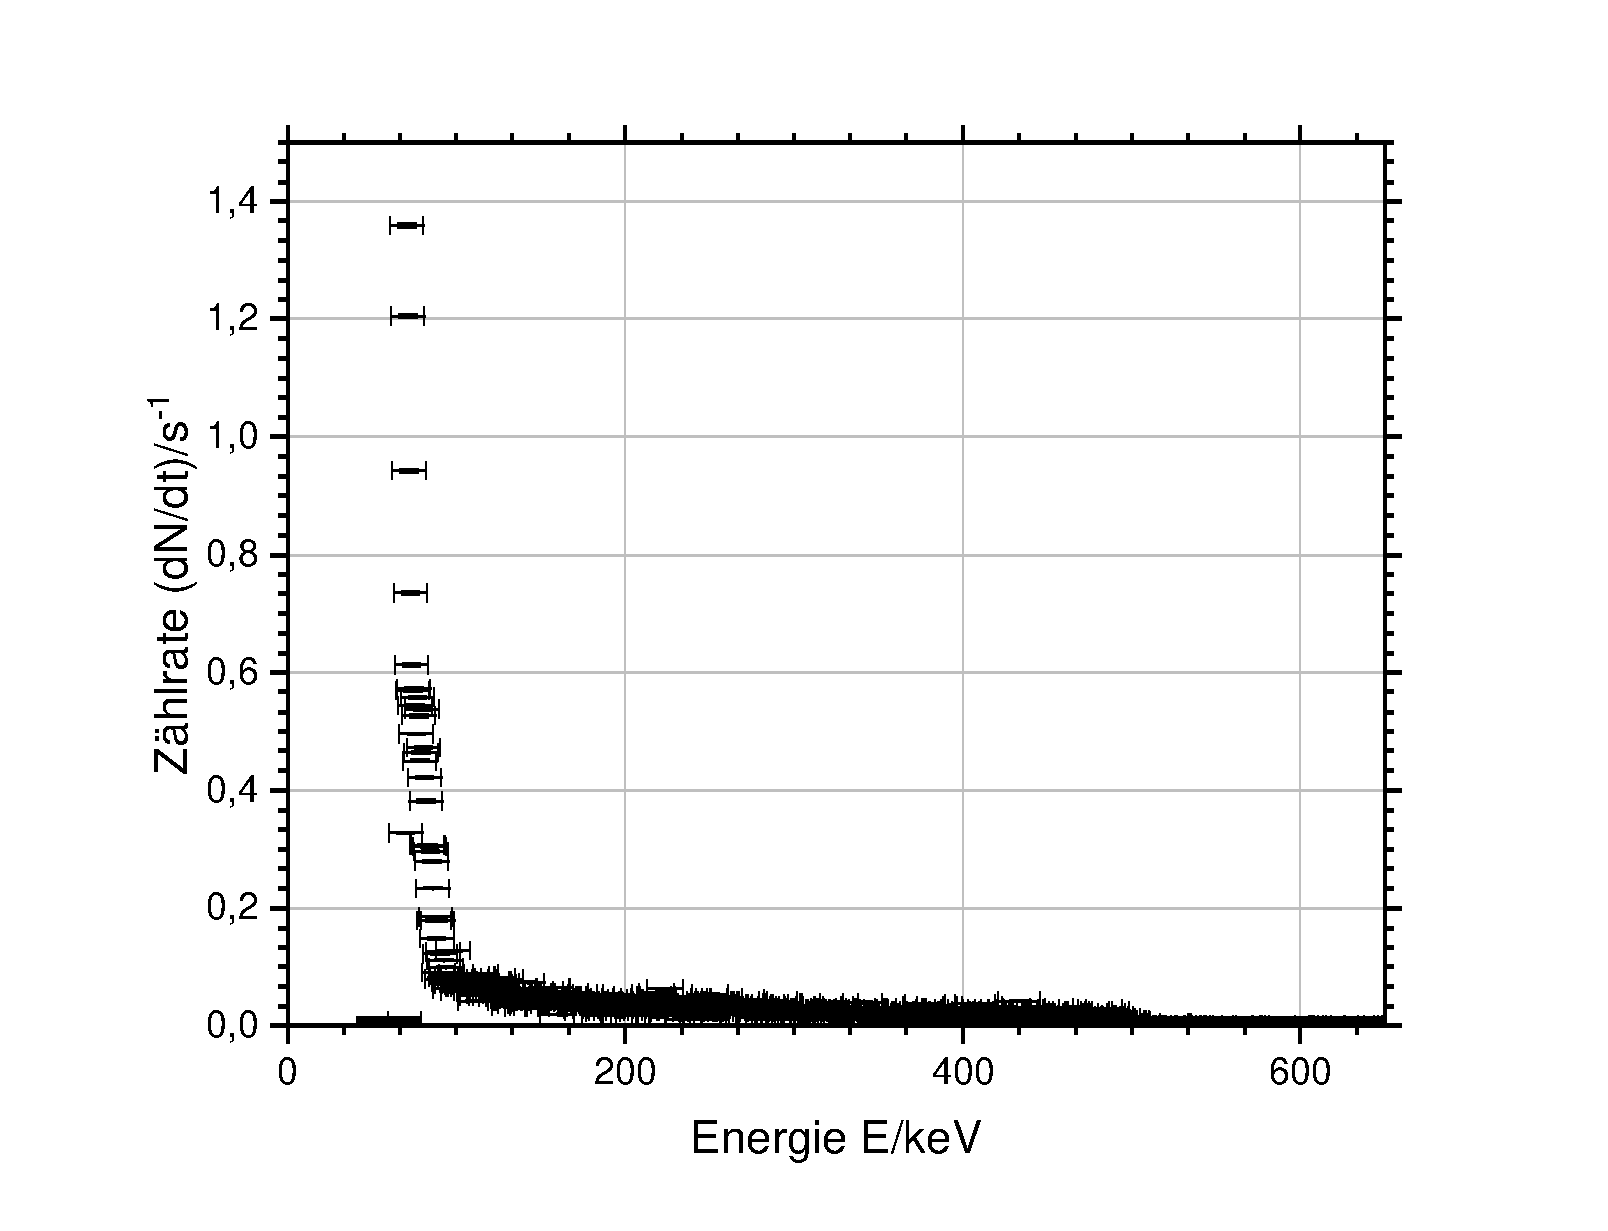
\includegraphics[width=\textwidth]{/home/tom/BE/Plots/CS_AL_plot_energie.pdf}
\captionof{figure}{\(\gamma\)-Spektrum von \(^{137}_{\ 55}\mathrm{Cs}\)}
%\end{flushleft}
\end{minipage}
%\begin{minipage}{0.04\textwidth}\centering
%\[\ \ \]
%\end{minipage}
\begin{minipage}{0.5\textwidth}\centering
%\begin{flushright}
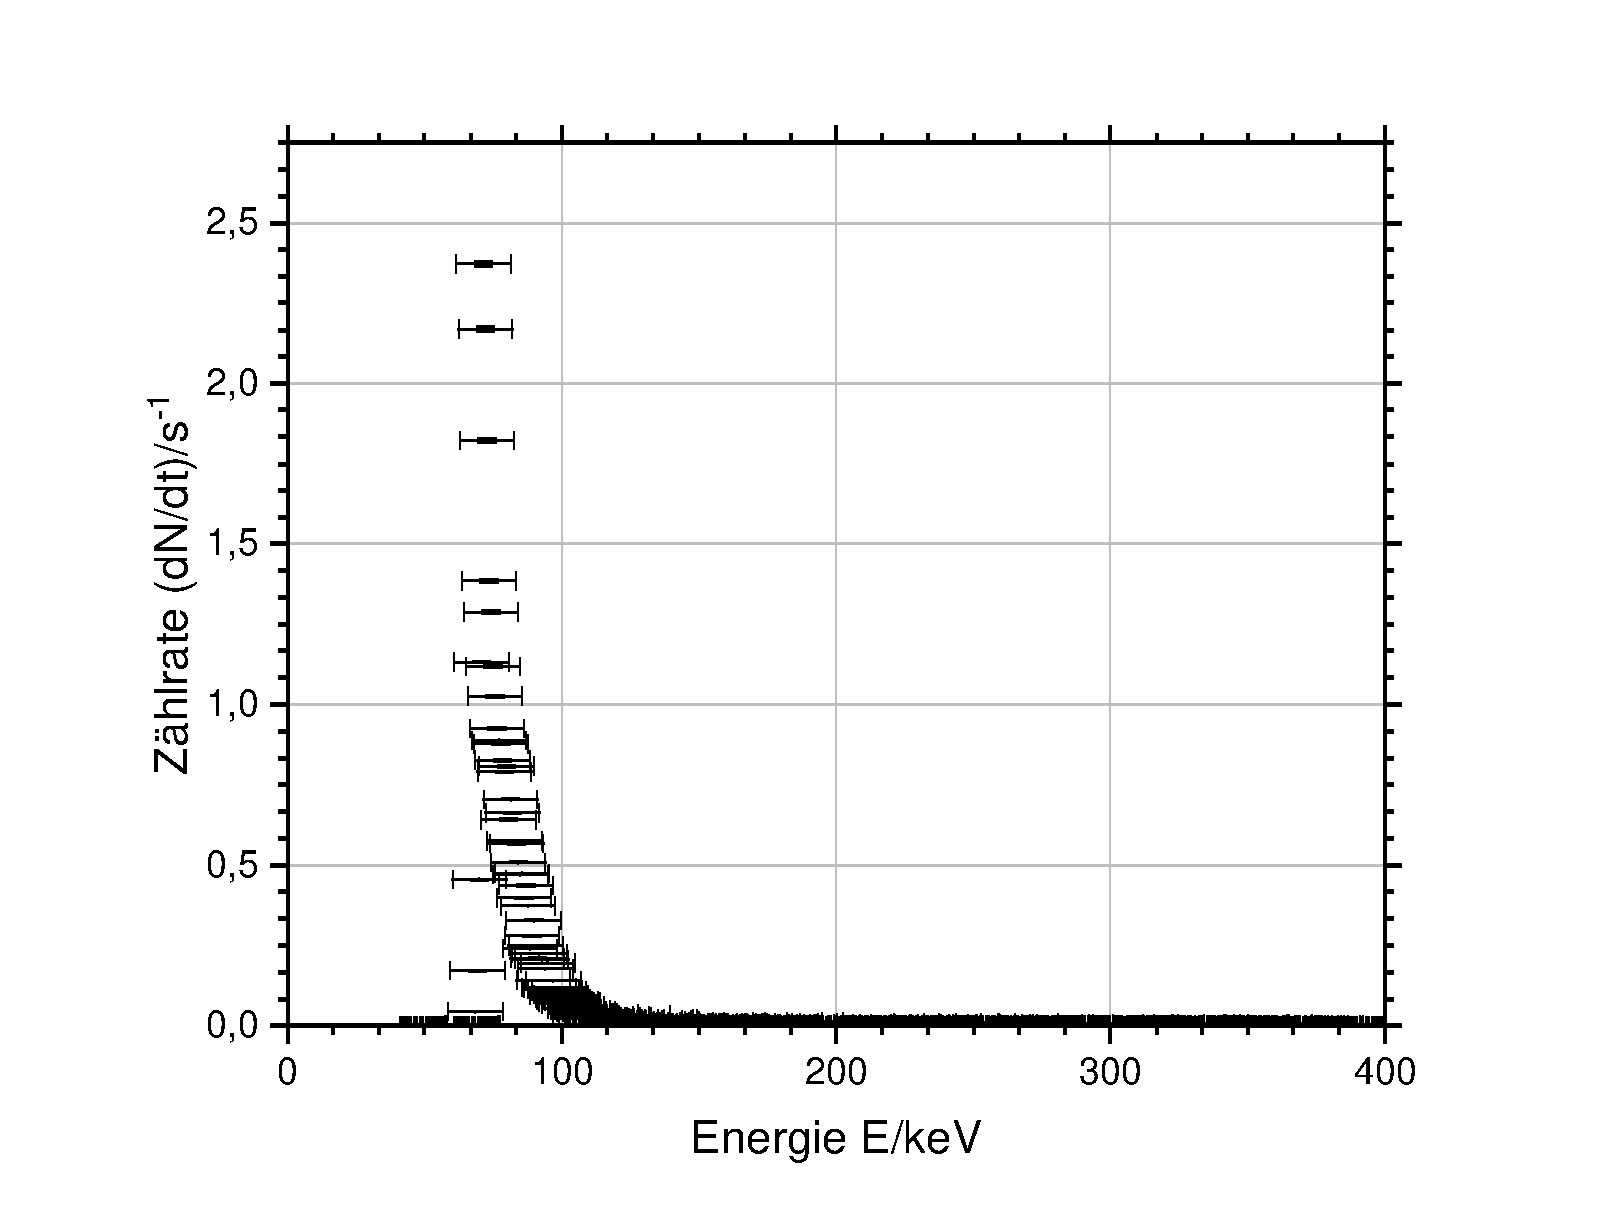
\includegraphics[width=\textwidth]{/home/tom/BE/Plots/KR_AL_plot_energie.pdf}
\captionof{figure}{\(\gamma\)-Spektrum von \(^{85}_{ 36}\mathrm{Kr}\)}
%\end{flushright}
\end{minipage} \\\\
\subsection{\(\beta^-\)-Spektren von \(^{137}_{\ 55}\mathrm{Cs}\) und \(^{85}_{36}\mathrm{Kr}\)}
Subtrahiert man den \(\gamma\)-Untergrund aus dem letzten Abschnitt vom Gesamtspektrum, erhält man das \(\beta^-\)-Spektrum des jeweiligen Nuklids. In Abb. 16 sowie Abb. 17 sind die Ergebnisse für beide Nuklide dargestellt.
\\
\begin{minipage}{0.5\textwidth}\centering
%\begin{flushleft}
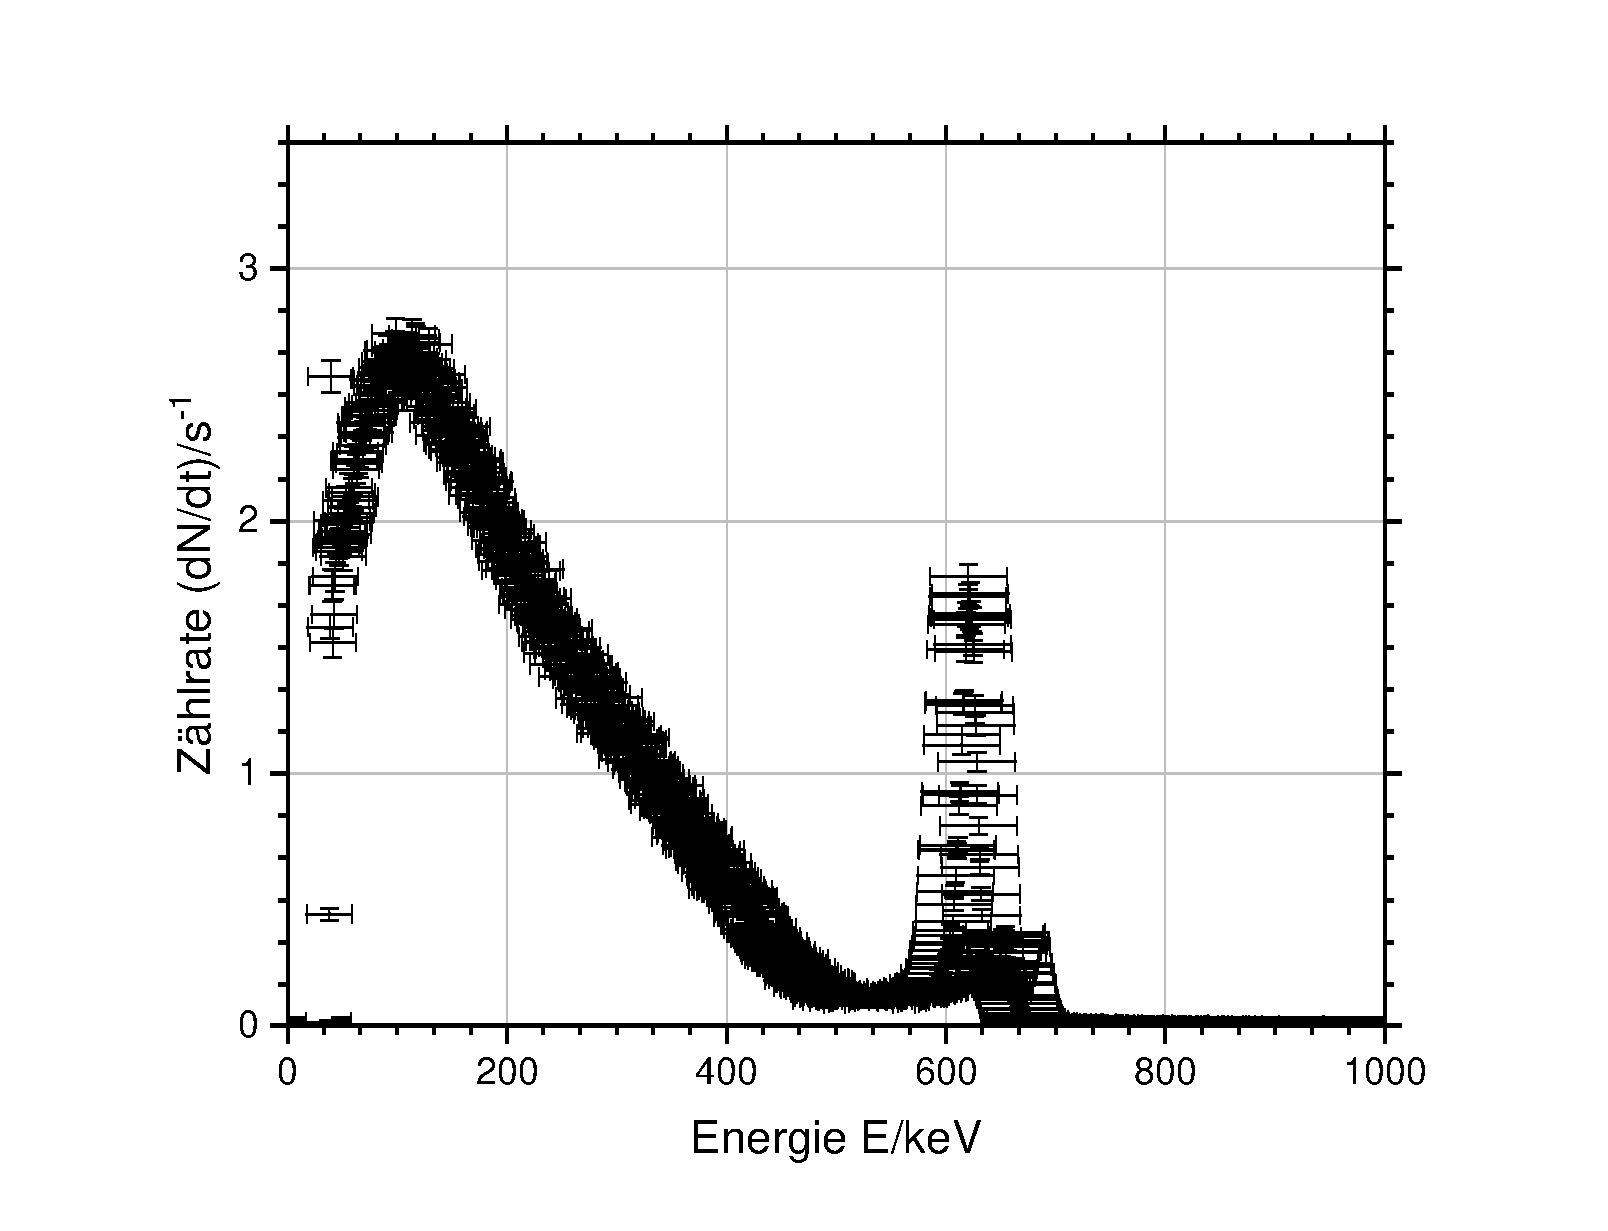
\includegraphics[width=\textwidth]{/home/tom/BE/Plots/CS_Spektrum.pdf}
\captionof{figure}{\(\beta^-\)-Spektrum von \(^{137}_{\ 55}\mathrm{Cs}\)}
%\end{flushleft}
\end{minipage}
%\begin{minipage}{0.04\textwidth}\centering
%\[\ \ \]
%\end{minipage}
\begin{minipage}{0.5\textwidth}\centering
%\begin{flushright}
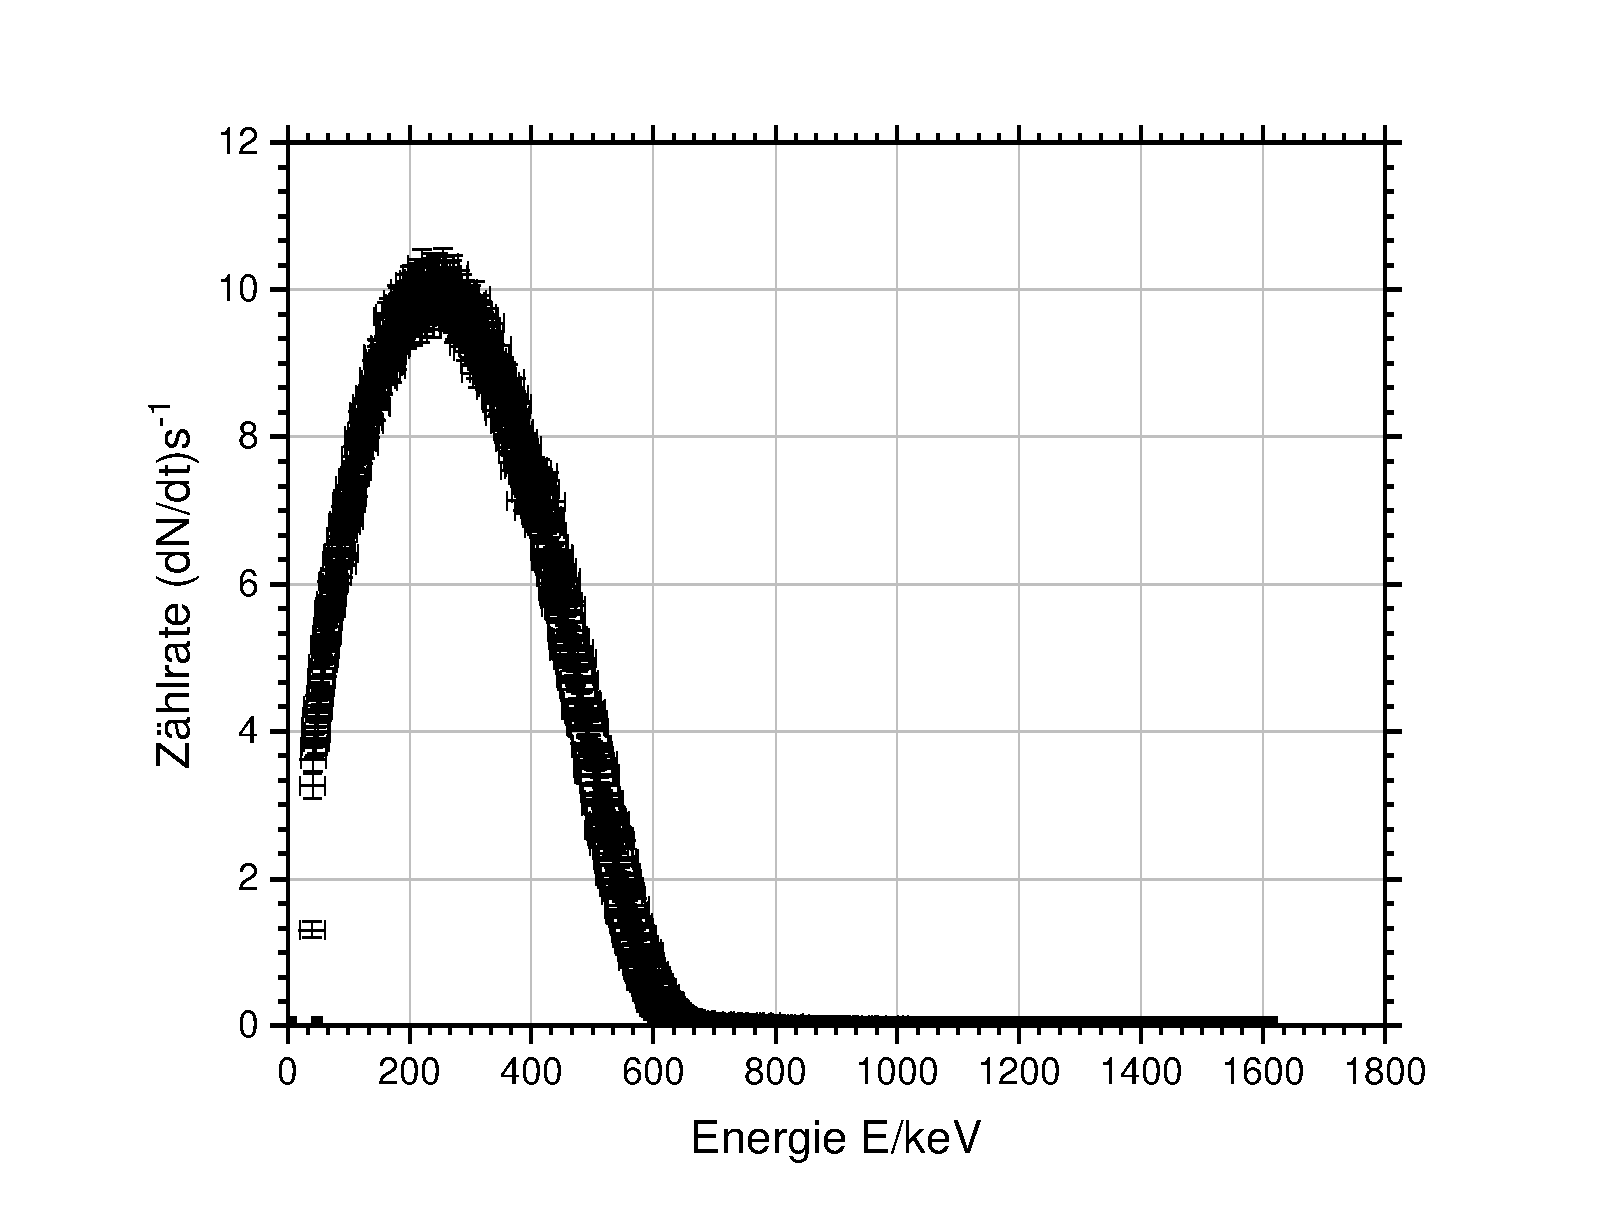
\includegraphics[width=\textwidth]{/home/tom/BE/Plots/KR_Spektrum.pdf}
\captionof{figure}{\(\beta^-\)-Spektrum von \(^{85}_{\ 36}\mathrm{Kr}\)}
%\end{flushright}
\end{minipage} \\\\
In beiden Fällen ist der kontinuierliche Verlauf des Spektrums deutlich zu erkennen. Dieser ist ein charakteristisches Merkmal von \(\beta\)-Übergängen, da es sich hier um einen Dreikörperzerfall handelt, bei dem Tochterkern und dem Elektron noch ein Elektron-Antineutrino frei wird. Im Gegensatz zu Zweikörperzerfällen, wie sie bei \(\alpha\)-Zerfall und \(\gamma\)-Übergängen typisch sind, sind damit die Energien und Impulse der einzelnen Zerfallsprodukte nicht eindeutig festgelegt. Dies äußert sich in einem kontinuierlichen Spektrum anstatt eines scharfen Linienspektrums. \\\\
Ein deutlicher Unterschied zwischen den Nukliden ist am Ende des Spektrums bei den energiereichsten Elektronen zu erkennen. Im Falle von \(^{137}_{\ 55}\mathrm{Cs}\) erhält man hier zwei sichtbare Peaks, die beim \(^{85}_{ 36}\mathrm{Kr}\) fehlen. Es handelt sich hierbei um die Konversionspeaks, die entstehen, wenn die Wellenfunktion des angeregten Kerns mit der Wellenfunktion kernnaher Elektronen überlappt und somit ein Übertrag der Anregungsenergie des Kerns auf die Elektronen stattfinden kann. Das unterschiedliche Verhalten lässt sich anhand der Übergangsschemata (Abb. 4) erklären: \(^{137}_{\ 55}\mathrm{Cs}\) geht nur in \(5.6\%\) der Fälle sofort in den Grundzustand von \(^{137}_{\ 56}\mathrm{Ba}\) über. In den übrigen \(94.4\%\) aller Fälle erhält man erst einen angeregten Bariumkern, sodass die Wahrscheinlichkeit für innere Konversion relativ hoch ist. Im Gegensatz dazu geht das \(^{85}_{36}\mathrm{Kr}\) in \(99.6\%\) der Fälle in den Grundzustand von \(^{85}_{37}\mathrm{Rb}\) über. Hier erhält man nur in \(0.4\%\) aller Fälle einen angeregten Kern, der dann zum Großteil durch "normale" \ \(\gamma\)-Übergänge anstatt durch innere Konversion in den Grundzustand übergeht. Wenn man eine Konversionswahrscheinlichkeit von etwa \(8\%\) wie beim \(^{137}_{\ 55}\mathrm{Cs}\) für die K-Schale veranschlagt, hätte man beim \(^{85}_{ 36}\mathrm{Kr}\) nur in etwa \(0.004\cdot 0.08 = 0.00032 \hat{=} 0.032\%\) aller Fälle einen K-Konversionübergang, wogegen man denselben beim \(^{137}_{\ 55}\mathrm{Cs}\) in etwa \(0.944\cdot 0.08 = 0.07520 \hat{=} 7.520\%\) aller Fälle erwartet. Selbst der wahrscheinlichste Konversionsübergang ist damit beim \(^{85}_{ 36}\mathrm{Kr}\) um mindestens einen Faktor 200 gegenüber dem von \(^{137}_{\ 55}\mathrm{Cs}\) unterdrückt und kann daher, falls vorhanden, nicht aufgelöst werden. Für die Berechnung von Konversionskoeffizienten eignet sich daher nur das Nuklid \(^{137}_{\ 55}\mathrm{Cs}\). 

\subsection{Auflösungsvermögen des Spektrometers}
Um das Auflösungsvermögen des Spektrometers zu beurteilen, wird die sogenannte Halbwertsbreite (FWHM) zu Rate gezogen. Sie ist für eine Gaußfunktion mit Standardabweichung $\sigma$ definiert als:
\begin{align*}
\text{FWHM} = 2\sqrt{2 \, \ln(2)} \cdot \sigma.
\end{align*}
Da allerdings für den Fit der Konversionspeaks (Abbildung 8) in der Fitfunktion der Parameter $w$ bereits diese Halbwertsbreite darstellt, kann diese nach Umrechnung in eine Energie für beide Peaks direkt angegeben werden:
\begin{align*}
\text{FWHM}@620.54\,\mathrm{keV} &= (15.02 \pm 0.74)\,\mathrm{keV} (\text{K-Schale}) \\
\text{FWHM}@653.68\,\mathrm{keV} &= (11.2 \pm 1.2)\,\mathrm{keV} (\text{L-Schale}) .
\end{align*}
Die beiden Halbwertsbreiten stimmen also nicht überein, da sie wie erwartet von der jeweiligen Energie abhängig sind. Deshalb ist zu jedem FWHM die zugehörige Energie angegeben.
\subsection{Konversionskoeffizienten von \(^{137}_{\ 55}\mathrm{Cs}\)}
Aus den Spektren von \(^{137}_{\ 55}\mathrm{Cs}\) können nun durch eine sorgfältige Analyse die Konversionskoeffizienten angegeben werden. Dazu werden die Zählraten im \(\gamma\)-Spektrum von \(E=0\) bis zur Compton-Kante zur Rate \(\dot{N}_{\gamma}\) addiert. Daneben werden die Raten für jeden einzelnen Konversionspeak zu \(\dot{N}_{\beta,\mathrm{K}}\) bzw. \(\dot{N}_{\beta,\mathrm{L}}\) aufaddiert. Die Konversionskoeffizienten sind definiert als Verhältnis der Konversionsübergange gegenüber einem Gammaübergang und berechnen sich damit zu:
\begin{align*}
\alpha_{\mathrm{K}} &= \frac{\dot{N}_{\beta,\mathrm{K}}}{\dot{N}_{\gamma}} = 8.60\% \\
\alpha_{\mathrm{L}} &= \frac{\dot{N}_{\beta,\mathrm{L}}}{\dot{N}_{\gamma}} = 1.65\% .
\end{align*}
Die Unsicherheiten der Zählraten ergeben sich nach der Poisson-Statistik in Kombination mit der Fehlerfortpflanzung nach Gauß zu
\begin{align*}
\Delta\dot{N} = \frac{\sqrt{N}}{t}.
\end{align*}
Sie können damit einfach berechnet werden. Es handelt sich hierbei um statistische Unsicherheiten, weil sie aus einer Zählstatistik stammen. Hinzu kommt noch eine systematische Unsicherheit, da sich bei der Auswertung gezeigt hat, dass das Ergebnis recht sensitiv davon abhängt, über welches Intervall der Peakbreite man integriert. Ferner hat der Detektor möglicherweise auch eine unterschiedliche Akzeptanz für Elektronen und Photonen. Wir veranschlagen hierfür aufgrund unserer Untersuchungen eine systematische Unsicherheit von etwa \(\Delta \alpha_{\mathrm{sys}} \approx 0.5\%\). Damit erhalten wir folgendes Ergebnis:
\begin{align*}
\text{Konversionskoeffizient K-Schale: } \alpha_{K} &= (8.60 \pm 0.50_{\mathrm{sys}} \pm 0.26_{\mathrm{stat}})\,\% \\
\text{Konversionskoeffizient L-Schale: } \alpha_{L} &= (1.65 \pm 0.50_{\mathrm{sys}} \pm 0.08_{\mathrm{stat}})\,\% .
\end{align*}
Im Vergleich mit den Literaturwerten 
\begin{align*}
\alpha_{\mathrm{K}} = 8.96\,\% \quad \text{und}\quad \alpha_{\mathrm{L}} = 1.67\,\%
\end{align*}
aus \cite{Anleitung} stimmen unsere Ergebnisse im Rahmen der Messgenauigkeit mit den empfohlenen Werten überein.
\subsection{Fermi-Plot und Grenzenergien}
Um die Maximalenergien der $\beta$-Teilchen zu bestimmen wird ein Fermi-Plot verwendet. Dazu trägt man den Asudruck
\begin{align*}
\text{N}_{\text{F}} := \sqrt{\frac{N(E)}{p\cdot W\cdot F(Z,E)}}
\end{align*}
über \(E_{\mathrm{kin}}\) der Elektronen aus der \(\beta^-\)-Strahlung auf. Es ergibt sich über einen weiten Bereich ein annähernd linearer Zusammenhang. Für diesen lässt sich eine Regressionsgerade bestimmen, die man dann in den Bereich der Konversionspeaks extrapolieren kann. Damit wird die Bestimmung der Maximalenergie der Elektronen aus dem \(\beta^-\)-Zerfall möglich, was normalerweise dadurch erschwert wird, dass die Konversionspeaks den interessierenden Bereich überdecken. Für $^{137}_{\ 55}$Cs ist der Übergang von den Messdaten zum Fermiplot in Abb. 18 gezeigt.
\newpage
\begin{figure}[h!]\centering
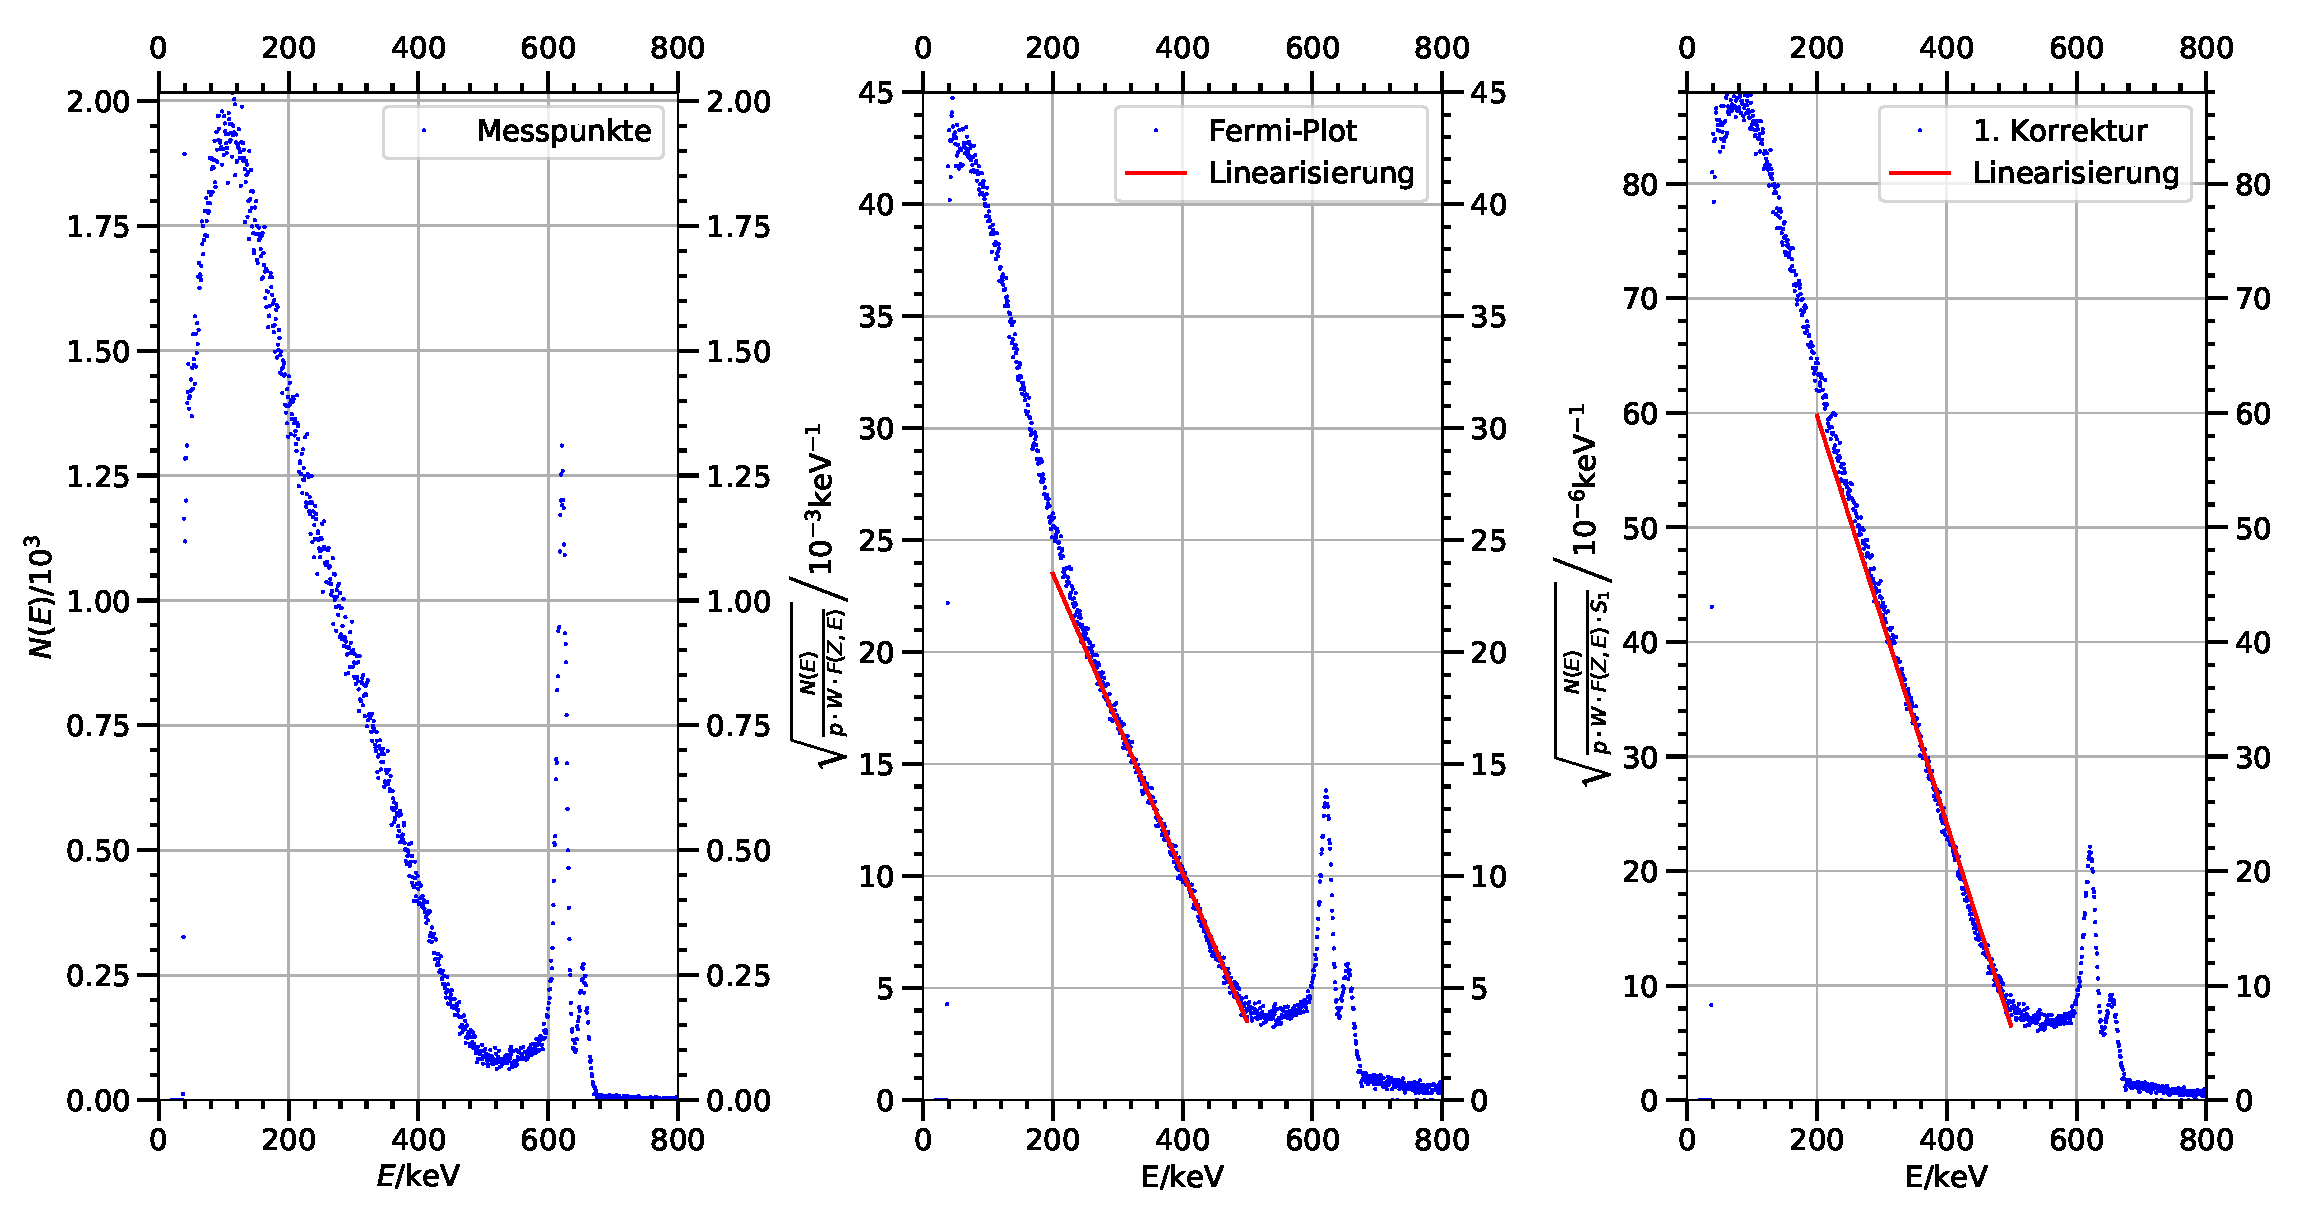
\includegraphics[width=\textwidth]{/home/tom/BE/Plots/Fermi_Plot_Cs_neu.pdf}
\caption{Im linken Diagramm ist nochmals das Spektrum von $^{137}_{\ 55}$Cs zu sehen. Das mittlere Diagramm zeigt den Fermi-Plot, in dem eine Linearisierung möglich ist. Durch Extrapolation erhält man die Maximalenergie \(E_0\) der Elektronen. Diese wurde im rechten Diagramm verwendet, um das Ergebnis iterativ zu verbessern (vgl. Erklärung unten).} 
\end{figure}
Für die Regressionsgerade wurden folgende Fitparameter bestimmt:
\begin{align*}
m &= (-668.0\pm 2.9_{\mathrm{stat}})\cdot 10^{-7}\,\frac{1}{\mathrm{keV^2}} \\
n &= (368.7\pm 1.3_{\mathrm{stat}})\cdot 10^{-4}\,\frac{1}{\mathrm{keV}}.
\end{align*}
Die Nullstelle der Gerade ergibt sich dann zu:
\begin{align*}
N_{\mathrm{F}}(E) = m\cdot E_0 + n \overset{!}{=} 0\quad\Longrightarrow\quad E_0 = -\frac{n}{m}.
\end{align*}
Damit erhält man als ersten Näherungswert für die Maximalenergie der Elektronen:
\begin{align*}
E_0 = (551.9\pm 3.1_{\mathrm{stat}})\,\mathrm{keV}
\end{align*}
Mit diesem Wert kann nun ein Korrekturfaktor
\begin{align*}
S_1 := (E+m_{\mathrm{e}})^2 - m_{\mathrm{e}} + (E_0-E)^2
\end{align*}
bestimmt werden, mit dem man die Fermifunktion auf \(F(Z,E) = F_{\mathrm{alt}}\cdot S_1 = 6\cdot S_1\) korrigiert. Trägt man das so korrigierte \(N_{\mathrm{F}}\) über \(E\) auf, erhält man das rechte Diagramm in Abb. 18. Ein erneuter linearer Fit ergibt dann einerseits
\begin{align*}
m &= (-1781.9\pm 9.2_{\mathrm{stat}})\cdot 10^{-10}\,\frac{1}{\mathrm{keV^2}} \\
n &= (954.1\pm 4.1_{\mathrm{stat}})\cdot 10^{-7}\,\frac{1}{\mathrm{keV}}.
\end{align*}
und damit die korrigierte Energie
\begin{align*}
E_0 = (535.4\pm 3.6_{\mathrm{stat}})\,\mathrm{keV}.
\end{align*}
Dasselbe Verfahren wird nun auch auf das Spektrum von \(^{85}_{36}\mathrm{Kr}\) angewendet. Die entstehenden Diagramme zeigt Abb. 19.\\\\
\begin{figure}[h!]\centering
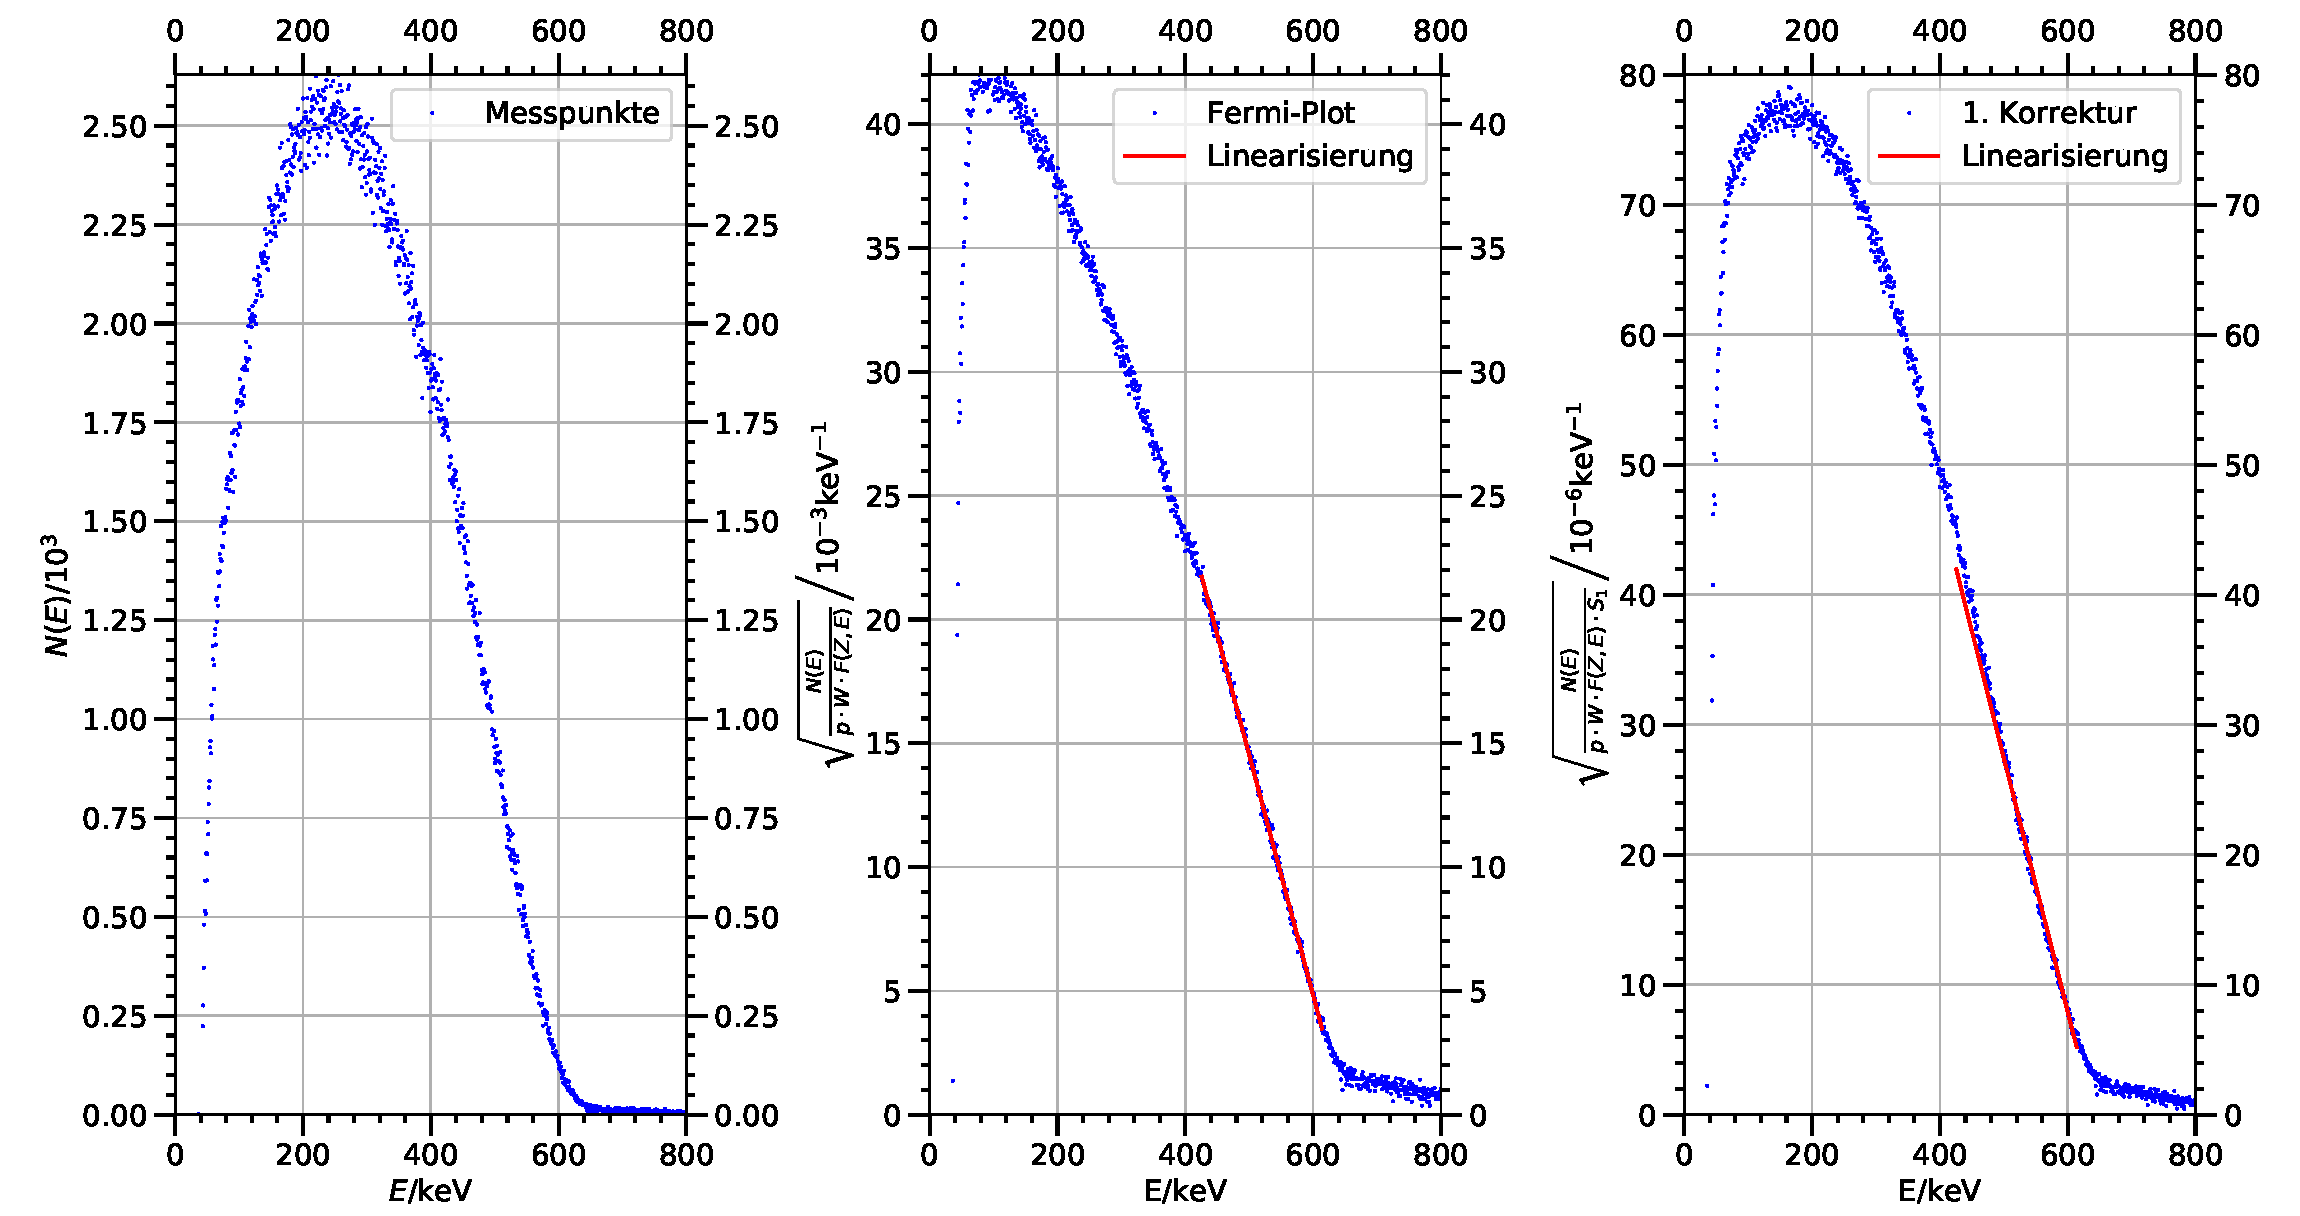
\includegraphics[width=\textwidth]{/home/tom/BE/Plots/Fermi_Plot_Kr_neu.pdf}
\caption{Linkes Diagramm: Spektrum von $^{85}_{36}$Kr. Mittleres Diagramm: Fermi-Plot desselben. Rechtes Diagramm: 1.Korrektur zum Fermiplot analog zu \(^{137}_{\ 55}\mathrm{Cs}\).} 
\end{figure}\\\\
Der lineare Fit im Fermiplot ergab zunächst folgende Werte für Anstieg, Achsenabschnitt und Maximalenergie der Elektronen:
\begin{align*}
m &= (-9.6\pm 3.6_{\mathrm{stat}})\cdot 10^{-5}\,\frac{1}{\mathrm{keV^2}} \\
n &= (630.0 \pm 2.0_{\mathrm{stat}})\cdot 10^{-4}\,\frac{1}{\mathrm{keV}} \\
E_0 &= (649.8\pm 3.2_{\mathrm{stat}})\,\mathrm{keV}.
\end{align*}
Mit einer analog zu \(^{137}_{\ 55}\mathrm{Cs}\) durchgeführten Korrektur 1. Ordnung ergeben sich folgende verbesserte Werte:
\begin{align*}
m &= (-195.1\pm 1.1_{\mathrm{stat}})\cdot 10^{-9}\,\frac{1}{\mathrm{keV^2}} \\
n &= (1250.4 \pm 6.3_{\mathrm{stat}})\cdot 10^{-7}\,\frac{1}{\mathrm{keV}} \\
E_0 &= (640.6\pm 4.8_{\mathrm{stat}})\,\mathrm{keV}.
\end{align*}
Da das Verfahren sensitiv darauf reagiert, welchen Bereich man für den linearen Fit verwendet, ist zusätzlich mit einer systematischen Unsicherheit zu rechnen, die wir hier durch Variation des Fitbereichs zu etwa \(\Delta_{\mathrm{sys}} E_0 \approx \pm 20.0\,\mathrm{keV}\) geschätzt haben. Damit lautet unser Ergebnis für die Maximalenergie der Elektronen aus der jeweils häufigsten \(\beta^-\)-Umwandlung im Zerfallsschema:
\begin{align*}
^{137}_{\ 55}\mathrm{Cs}:\quad E_0 &= (535.4\pm 20.0_{\mathrm{sys}} \pm 3.6_{\mathrm{stat}})\,\mathrm{keV} \\
^{85}_{36}\mathrm{Kr}:\quad E_0 &= (640.6\pm 20.0_{\mathrm{sys}} \pm  4.8_{\mathrm{stat}})\,\mathrm{keV}.
\end{align*}
Die verwendete Literatur \cite{Anleitung} empfiehlt einen Wert von \(513.97\,\mathrm{keV}\) für \(^{137}_{\ 55}\mathrm{Cs}\) bzw. \(687.1\,\mathrm{keV}\) für \(^{85}_{36}\mathrm{Kr}\), wie man dem Zerfallsschema in Abb. 4 entnehmen kann. Unsere Messung liefert im Rahmen der Messgenauigkeit und der Unsicherheiten bei der linearen Anpassung vergleichbare Ergebnisse. \\\\
Für \(^{137}_{\ 55}\mathrm{Cs}\) ist der direkte Übergang in den Grundzustand mit einer Energie von \(1175.63\,\mathrm{keV}\) nicht sichtbar, weil er nur eine relative Häufigkeit von etwa \(5.6\,\%\) hat und daher vom Übergang in den angeregten Zustand mit anschließendem \(\gamma\)-Übergang überdeckt wird. Ebenso ist beim \(^{85}_{36}\mathrm{Kr}\) der \(173.1\,\mathrm{keV}\)-Übergang in den angeregten Zustand mit nur \(0.4\,\%\) relativer Häufigkeit gegenüber dem direkten Übergang in den Grundzustand unterdrückt. Das gesamte Zerfallsschema lässt sich allein mit dem Fermi-Plot nicht rekonstruieren; hierfür muss das \(\gamma\)-Spektrum inklusive innerer Konversion gemessen werden und dann die Differenz zwischen angergtem Zustand des Tochterkerns und Energie des Mutterkerns berechnet werden. 
\subsection{Wechselwirkung von \(\beta\)-Strahlung mit Materie}
\subsubsection{Energieverlust der Strahlung beim Durchgang durch Aluminium}
Im Versuch wurden Spektren von \(\beta^-\)-Strahlung beim Durchdringen von Papier und dünner Aluminiumfolie aufgenommen. Anhand dieser Messung lässt sich die Wechselwirkung von Elektronen mit Materie studieren und mit gängigen Theorie vergleichen. Eine in der Teilchenphysik oft benutzte Theorie verwendet die Bethe-Bloch-Formel, die beim Durchgang durch Materie einen mittleren Energieverlust von
\begin{align*}
\left \langle \frac{\mathrm{d}E}{\mathrm{d} x} \right \rangle= -\rho
z^2 \frac{K}{2} \frac{Z}{A} \frac{1}{\beta^2} \left[ \ln \left(\frac{\tau^2(\tau+2)}{2I/(m_{\mathrm{e}}^2)}\right)+F(\tau)- \delta(\beta \gamma)\right]
\end{align*}
voraussagt und voll-relativistisch formuliert ist. Multiplikation mit \(\langle\mathrm{d}x\rangle\) ergibt dann:
\begin{align*}
\langle \mathrm{d}E  \rangle &= -\rho\langle\mathrm{d} x\rangle 
z^2 \frac{K}{2} \frac{Z}{A} \frac{1}{\beta^2} \left[ \ln \left(\frac{\tau^2(\tau+2)}{2I/(m_{\mathrm{e}}^2)}\right)+F(\tau)- \delta(\beta \gamma)\right] \\
&= \bar{\rho}\cdot 
z^2 \frac{K}{2} \frac{Z}{A} \frac{1}{\beta^2} \left[ \ln \left(\frac{\tau^2(\tau+2)}{2I/(m_{\mathrm{e}}^2)}\right)+F(\tau)- \delta(\beta \gamma)\right] 
\end{align*}
wobei mit \(\bar{\rho}=\rho\langle\mathrm{d} x\rangle \) die Flächenmasse eingeführt wurde, die für die hier verwendete Aluminiumfolie bei etwa \(\bar{\rho} = 2.7\,\frac{\mathrm{mg}}{\mathrm{cm}^2}\) liegt. Für die Elektronen des K-Konversionspeaks von \(^{137}_{\ 55}\mathrm{Cs}\) ist \(E_{\mathrm{kin}}= E^\mathrm{K}_{\mathrm{IC}} = 624.219\,\mathrm{keV}\), wie in der Kalibrierung gezeigt. Daraus erhält man
\begin{align*}
\gamma &= \frac{E_{\mathrm{kin}}}{m} + 1 = \frac{624.219\,\mathrm{keV}}{510.999\,\mathrm{keV}} + 1 = 2.222 \\
\beta &= \sqrt{\frac{\gamma^2 - 1}{\gamma^2}} = \sqrt{\frac{2.222^2 - 1}{2.222^2}} = 0.893 \\
\Longrightarrow\quad \tau &:= \gamma -1 = 1.222\quad\text{und}\quad F(\tau) := 1 - \beta^2 + \frac{\frac{\tau^2}{8} - \ln 2(2\tau+1)}{(\tau + 1)^2} = -0.151.
\end{align*}
Ferner ist bei Elektronen \(z=-1\) sowie für Aluminium \(Z=13\), \(A=27\), \(I=150\,\mathrm{eV}\). \(K\approx0.3071\,\frac{\mathrm{MeV}\cdot\mathrm{cm^2}}{\mathrm{mol}}\) ist eine Konstante und \(\delta(\beta\gamma)\) ist für die hier betrachtete Energie vernachlässigbar; dieser Polarisationsverlust spielt erst für \(E_{\mathrm{kin}} \geq 1\,\mathrm{MeV}\) eine Rolle (vgl. \cite{Anleitung}). 
Man erhält damit:
\begin{align*}
\langle \mathrm{d}E  \rangle = \bar{\rho}\cdot 
z^2 \frac{K}{2} \frac{Z}{A} \frac{1}{\beta^2} \left[ \ln \left(\frac{\tau^2(\tau+2)}{2I/(m_{\mathrm{e}}^2)}\right)+F(\tau)- \delta(\beta \gamma)\right] \approx -5.5084\,\mathrm{keV}\cdot \bar{\rho} 
\end{align*}
Das ist die mittlere Energieänderung der Elektronen, wenn sie eine Schicht der Dicke \(\mathrm{d}x\) aus einem Material der Dichte \(\rho\) oder modellhaft einer dünnen Folie der Flächenmasse \(\bar{\rho}\) durchquert haben. Da die K-Konversionselektronen eine Anfangsenergie von \(E=624.219\,\mathrm{keV}\) haben, lautet die Energie nach durchqueren der dünnen Schicht 
\begin{align*}
\underline{\underline{E(\bar{\rho}) = 624.219\,\mathrm{keV} - 5.508\,\mathrm{keV}\cdot \bar{\rho}}}.
\end{align*}
Eine analoge Rechnung lässt sich nun auch für das Landau-Modell durchführen. Dieses berechnet den mittleren Energieverlust bei einer Wegstrecke \(x\) gemäß:
\begin{align*}
\Delta E =z^2 \frac{K}{2} \frac{Z}{A} \frac{\rho}{\beta^2}x \left[ \ln \left(\frac{KZm_{\mathrm{e}}\rho}{2I^2(1-\beta^2)A}x\right)- \beta^2- \delta(\beta \gamma)\right].
\end{align*}
Interpretiert man abermals \(\rho\cdot x = \bar{\rho}\) als Flächenmasse und setzt alle Werte ein, erhält man:
\begin{align*}
\Delta E = 0.2503386\,\mathrm{keV}\cdot \bar{\rho}\left[\ln(8286772\cdot \bar{\rho}) - 0.797 \right].
\end{align*}
Da die Schichtdicke nur wenig variiert wird und der Logarithmus extrem langsam wächst, ist es im hier betrachteten Rahmen erlaubt \(\bar{\rho}\ln(a\cdot \bar{\rho})\approx \ln(a)\bar{\rho}\) zu setzen. Einsetzen dieser Näherung ergibt dann:
\begin{align*}
\Delta E(\bar{\rho}) \approx 0.2503386\,\mathrm{keV}\cdot \bar{\rho}\left[\ln(8286772) - 0.797 \right] = 3.788\,\mathrm{keV}\cdot \bar{\rho}.
\end{align*}
Dies ist der mittlere Energie, den das Landau-Modell pro Schicht vorhersagt. Mit der Anfangsenergie von \(624.219\,\mathrm{keV}\) ergibt sich damit folgender Zusammenhang zwischen Energie und Flächenmasse:
\begin{align*}
\underline{\underline{ E(\bar{\rho}) = 624.219\,\mathrm{keV} - 3.788\,\mathrm{keV}\cdot \bar{\rho}}}.
\end{align*}
Beide Modelle sagen einen affin-linearen Zusammenhang zwischen der Energie und der Schichtdicke vorher, zumindest in erster Näherung. Das Landau-Modell ergibt einen geringeren Energieverlust pro Schicht, als das Bethe-Bloch-Modell. Der Vergleich der experimentellen Messwerte mit den Modellen nach Bethe-Bloch und nach Landau ist in Abb. 20 dargestellt. \\\\
\begin{figure}[h!]\centering
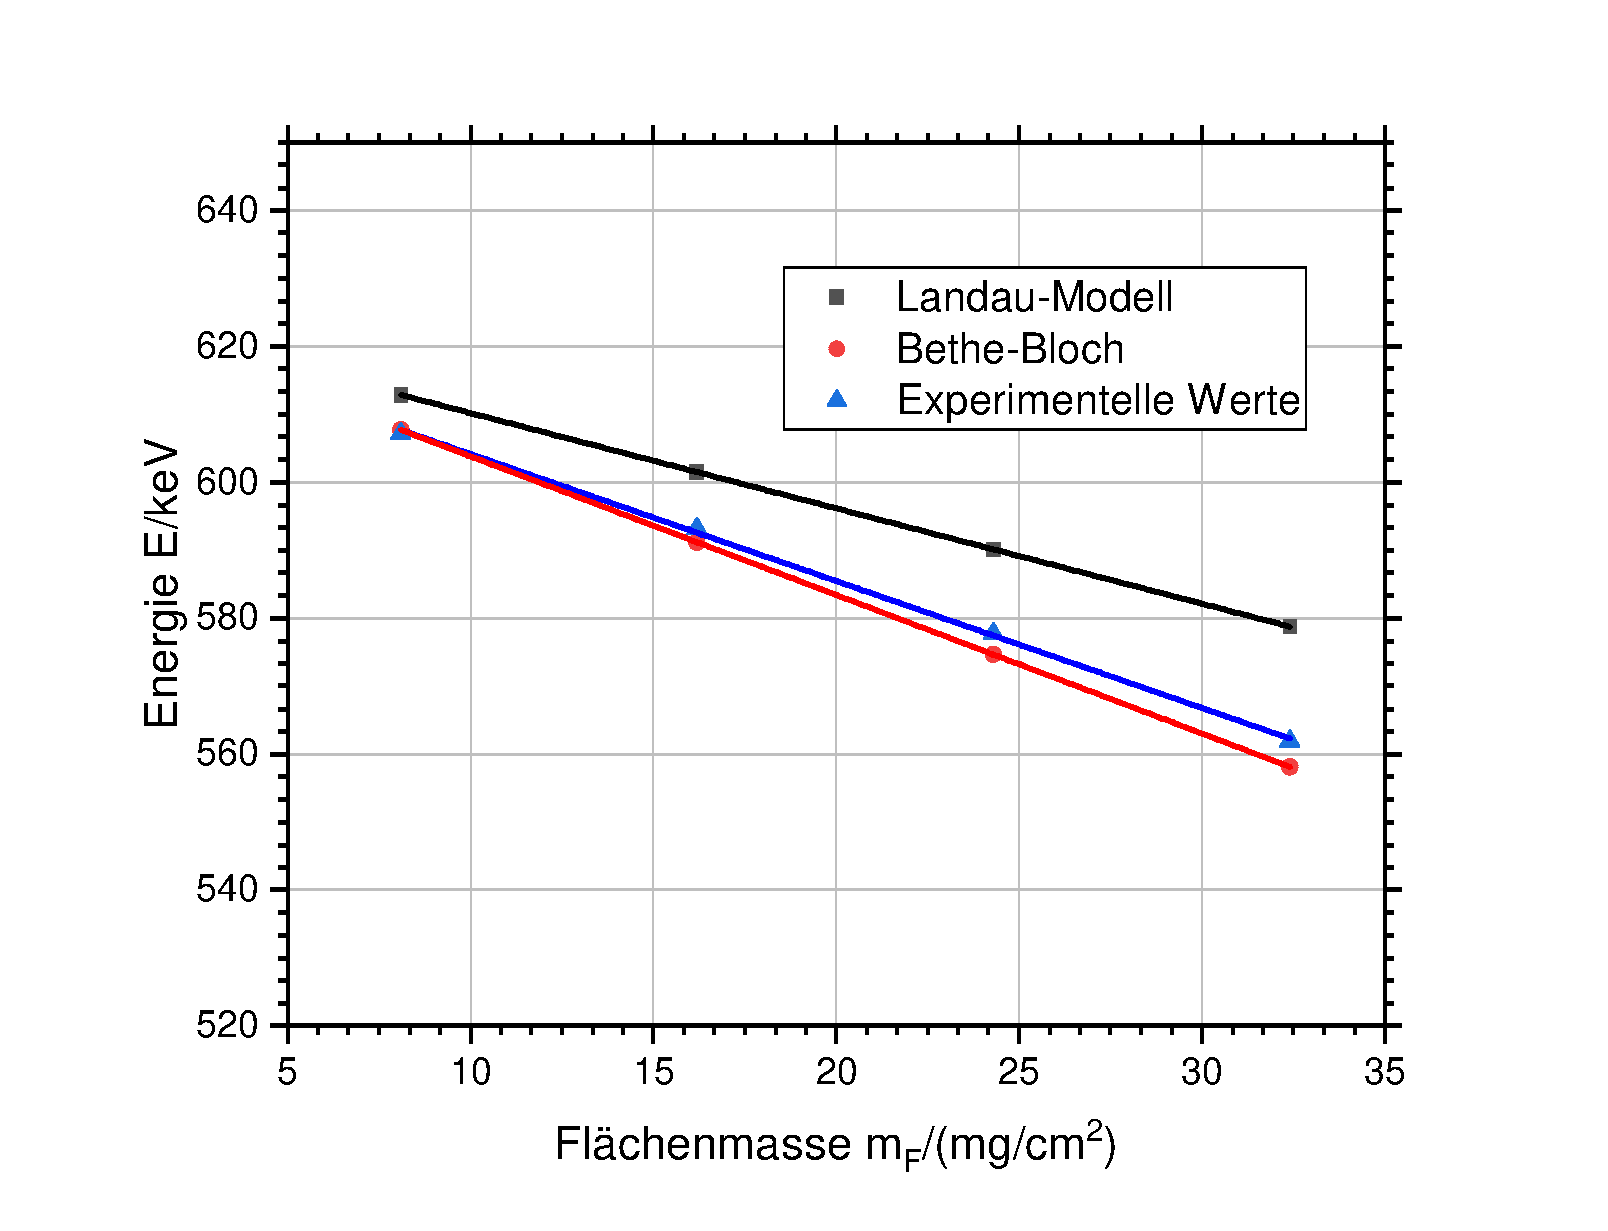
\includegraphics[width=\textwidth]{/home/tom/BE/Plots/bethe_bloch_landau.pdf}
\caption{Energieverlust der \(\beta^-\)-Strahlung in Abhängigkeit von der Schichtdicke für Aluminium. Vergleich zwischen experimentellen Daten und den Modellen nach Landau sowie nach Bethe-Bloch.}
\end{figure} \\\\
Die Messwerte liegen wie erwartet zwischen den beiden Modellen. Das Bethe-Bloch-Modell sagt den Energieverlust etwas zu groß voraus. Da die experimentellen Werte sehr nahe an der Bethe Bloch-Formel liegen, wäre es naheliegend, dass die Abweichung möglicherweise durch den Polarisationsverlust erklärt werden kann, der allerdings schwer zugänglich ist. Das Landau-Modell sagt dagegen einen zu geringen Energieverlust voraus. Ein wesentlicher Unterschied zwischen den beiden Modellen liegt darin, dass das Modell von Landau den wahrscheinlichsten, d.h. in einem Ensemble am häufigsten auftretenden Energieverlust berechnet, das Modell von Bethe-Bloch dagegen den gemittelten Energieverlust. Insgesamt passt das Bethe-Bloch-Modell aber besser zu den gemessenen Werten.
\subsubsection{Absorption von \(\beta^-\)-Strahlung}
Anhand der experimentellen Daten lässt sich auch etwas über die Absorption der \(\beta^-\)-Strahlung aussagen. Dazu betrachtet man das kontinuierliche Spektrum nach dem Durchgang durch ein Stück Materie, welches die Energieverteilung im Ensemble von Teilchen darstellt, und integriert von null bis zu einer variablen oberen Energie. Die Darstellung über der Flächenmasse von Aluminium bzw. Papier ergibt dann die Energieabsorption in Abhängigkeit von der Schichtdicke. Durch die Integration wird die statistische Verteilung der einzelnen Energien in Form einer Ensemblemittelung berücksichtigt. Die sich ergebende funktionale Abhängigkeit ist in Abb. 21 bis Abb. 24 dargestellt.\\
\begin{minipage}{0.5\textwidth}\centering
%\begin{flushleft}
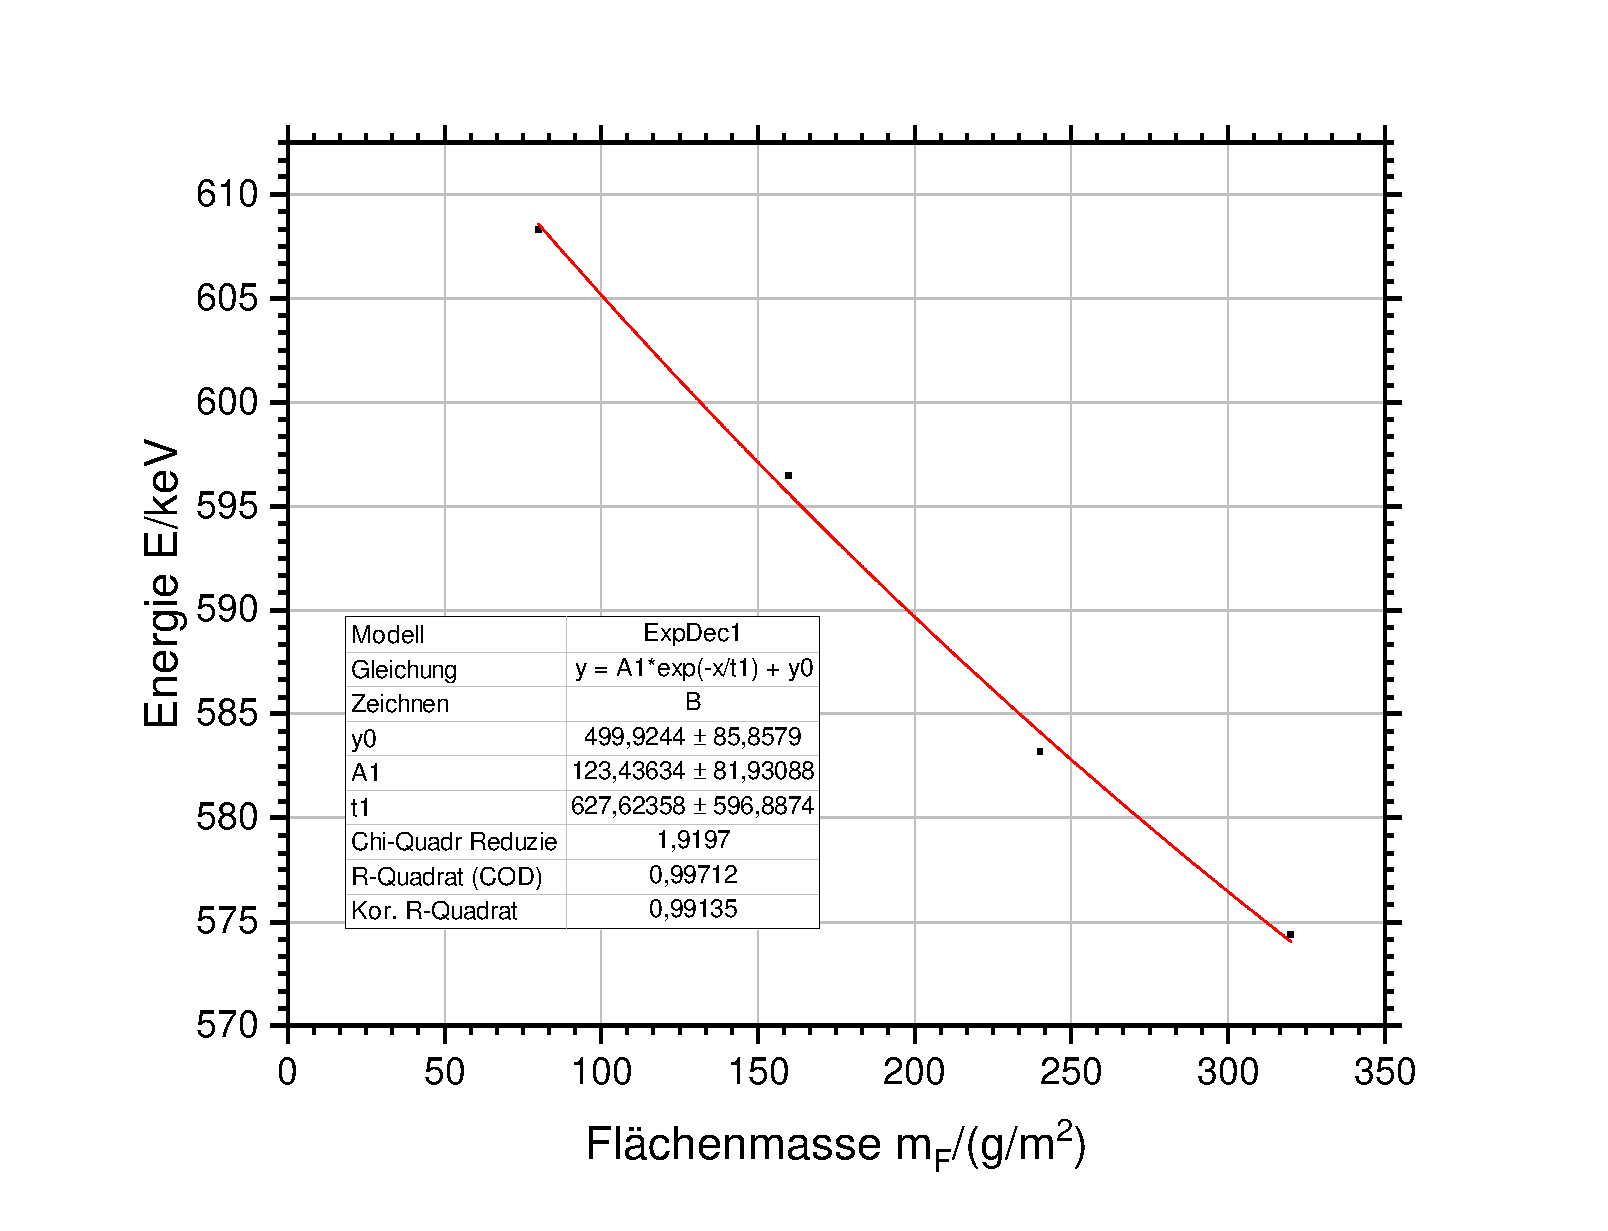
\includegraphics[width=\textwidth]{/home/tom/BE/Plots/CS_Papier.pdf}
\captionof{figure}{Absorption von \(\beta^-\)-Strahlung \\ in Papier für $^{137}_{\ 55}$Cs}
%\end{flushleft}
\end{minipage}
%\begin{minipage}{0.04\textwidth}\centering
%\[\ \ \]
%\end{minipage}
\begin{minipage}{0.5\textwidth}\centering
%\begin{flushright}
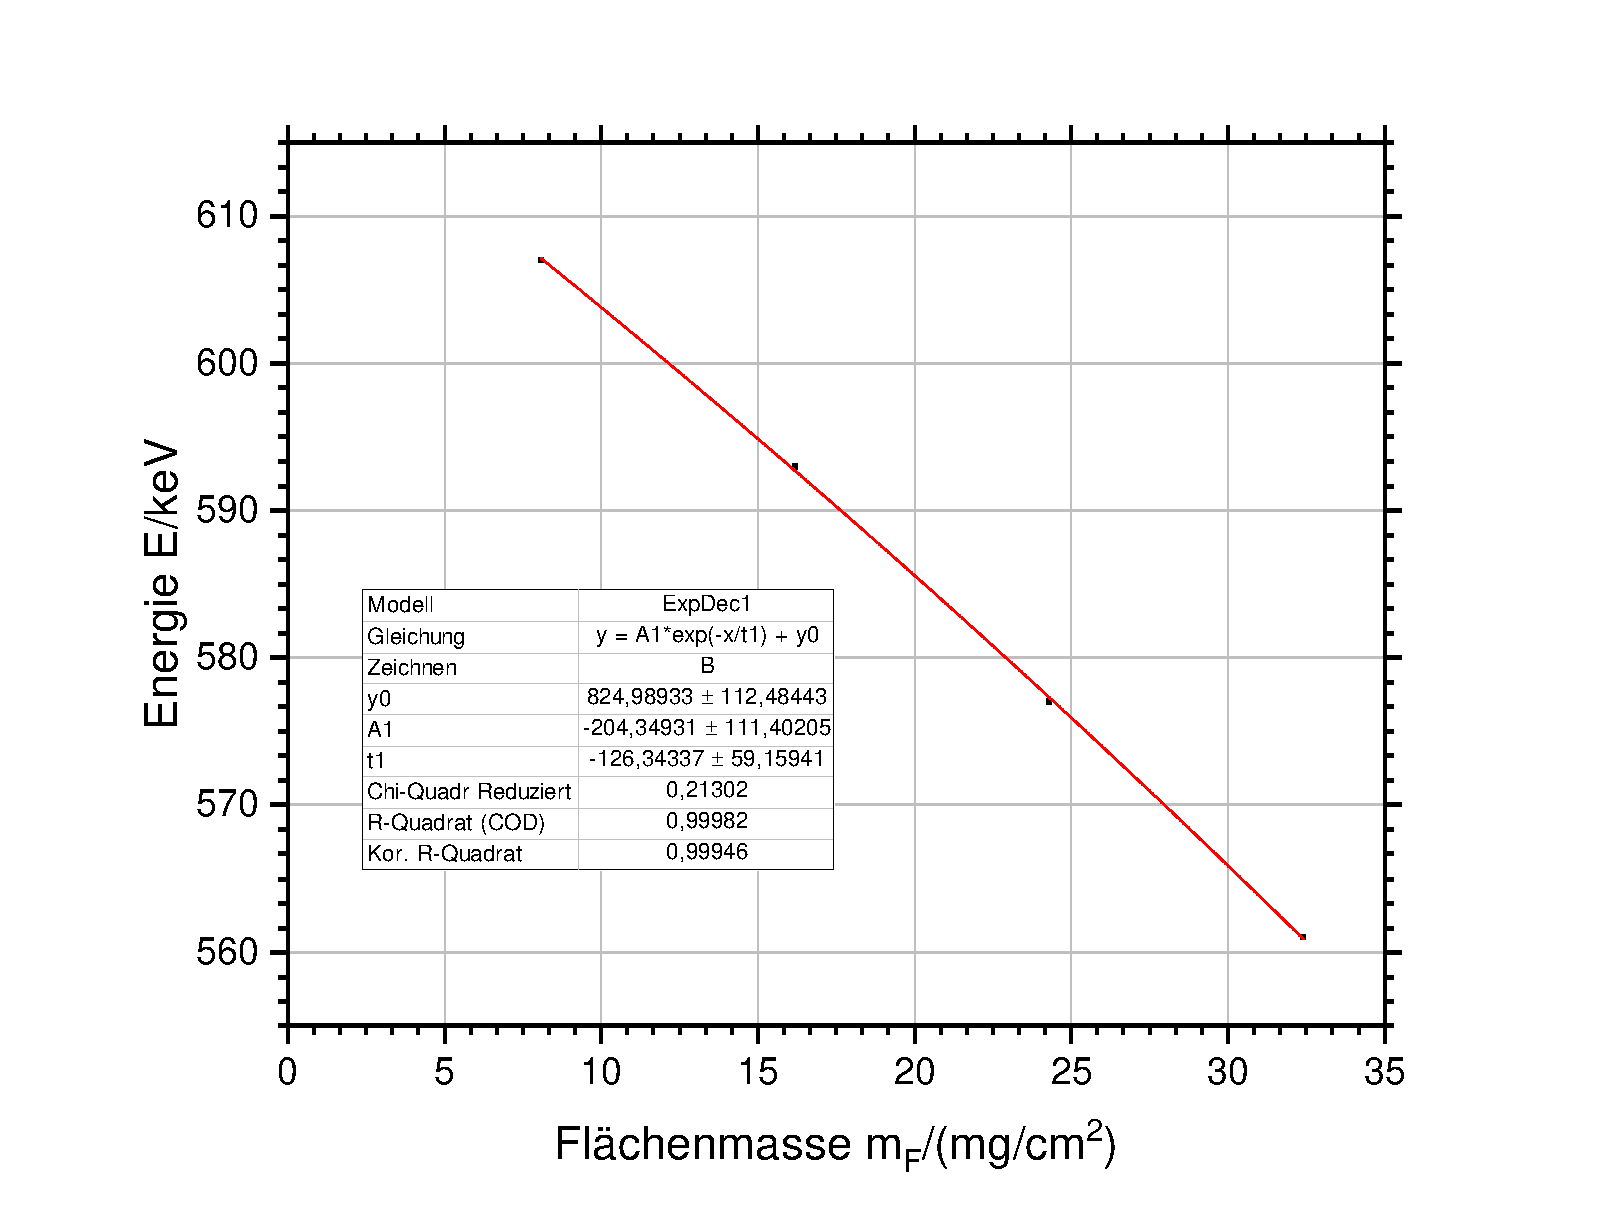
\includegraphics[width=\textwidth]{/home/tom/BE/Plots/CS_Al.pdf}
\captionof{figure}{Absorption von \(\beta^-\)-Strahlung \\ in Aluminium für $^{137}_{\ 55}$Cs }
%\end{flushright}
\end{minipage} \\\\
\begin{minipage}{0.5\textwidth}\centering
%\begin{flushleft}
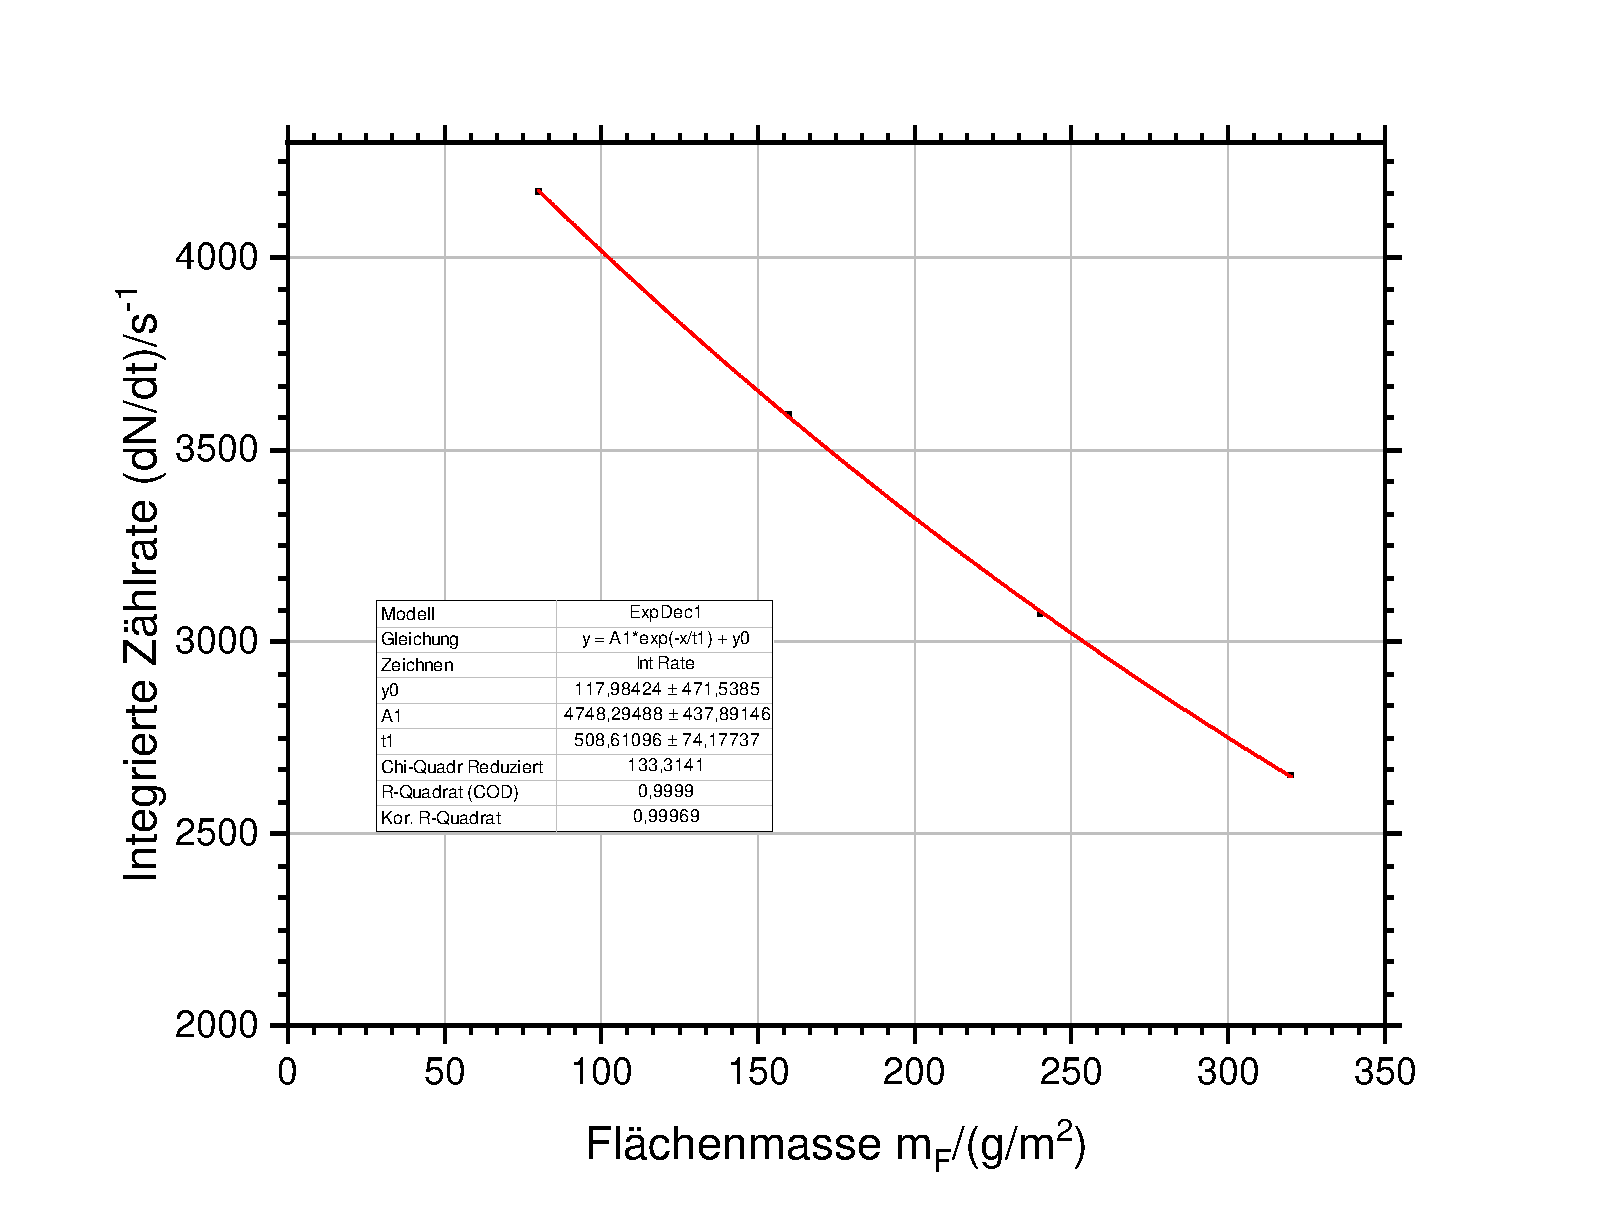
\includegraphics[width=\textwidth]{/home/tom/BE/Plots/KR_Papier.pdf}
\captionof{figure}{Absorption von \(\beta^-\)-Strahlung \\ in Papier für $^{85}_{36}$Kr }
%\end{flushleft}
\end{minipage}
%\begin{minipage}{0.04\textwidth}\centering
%\[\ \ \]
%\end{minipage}
\begin{minipage}{0.5\textwidth}\centering
%\begin{flushright}
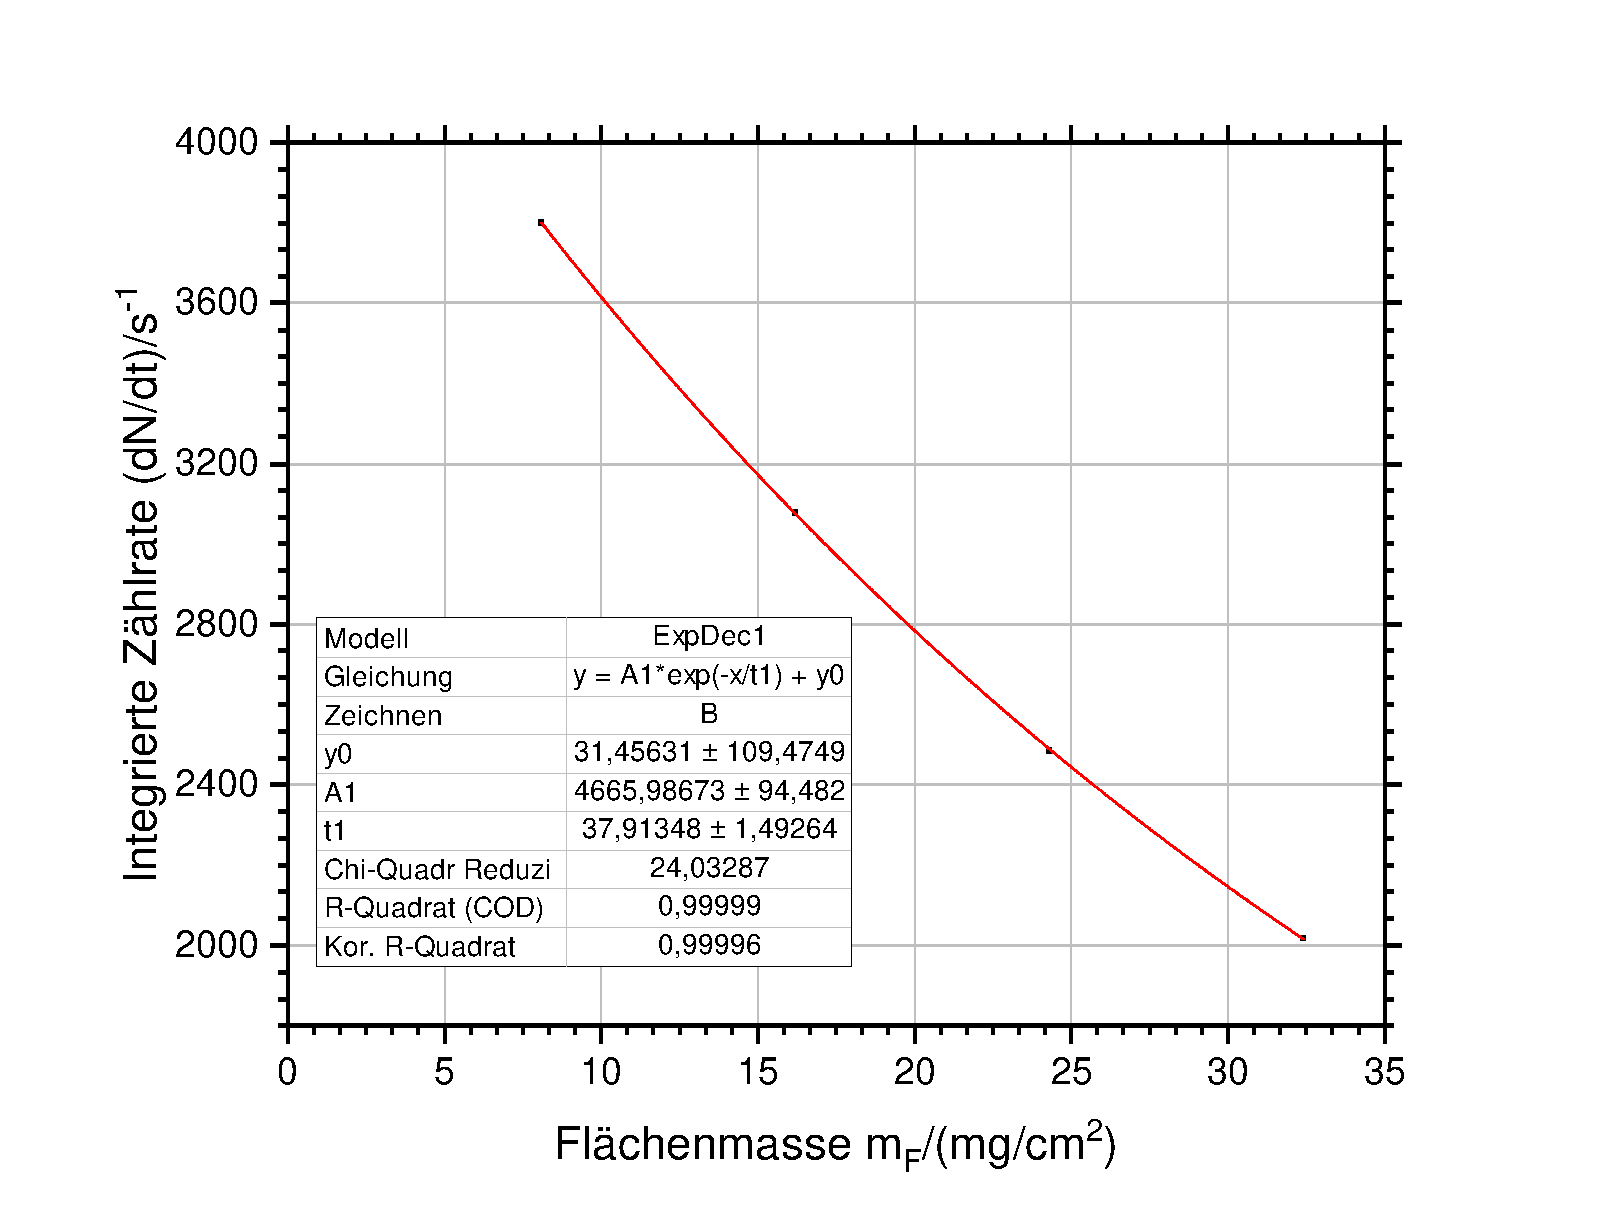
\includegraphics[width=\textwidth]{/home/tom/BE/Plots/KR_Al.pdf}
\captionof{figure}{Absorption von \(\beta^-\)-Strahlung \\ in Aluminium für $^{85}_{36}$Kr }
%\end{flushright}
\end{minipage} \\\\
Die Messwerte folgen in allen vier Fällen in sehr guter Näherung einem exponentiellen Schwächungsgesetz. Es ist daher leicht möglich, einen charakteristischen Schwächungskoeffizienten anzugeben, für den die transmittierende Strahlung auf den Anteil \(\frac{1}{\mathrm{e}}\) abgefallen ist. Durch einen exponentiellen Fit ergeben sich folgende Koeffizienten:
\begin{align*}
\underline{^{137}_{\ 55}\mathrm{Cs}:} \quad \mu_{\mathrm{Papier}} &= (0.0016 \pm 0.0016)\,\frac{\mathrm{cm}^2}{\mathrm{g}}\\
\mu_{\mathrm{Al}} &= (0.0079 \pm 0.0037)\,\frac{\mathrm{cm}^2}{\mathrm{g}} \\
\underline{^{85}_{36}\mathrm{Kr}:} \quad\mu_{\mathrm{Papier}} &= (0.00197 \pm 0.00029)\,\frac{\mathrm{cm}^2}{\mathrm{g}} \\
\mu_{\mathrm{Al}} &= (0.0264 \pm 0.0010)\,\frac{\mathrm{cm}^2}{\mathrm{g}} \\
\end{align*}
In beiden Fällen hat Aluminium den höheren Schwächungskoeffizienten. Deshalb fällt dort die Intensität der \(\beta^-\)-Strahlung wesentlich schneller ab, sodass sich Aluminium besser als Papier zur Abschirmung eignet. Für das Nuklid \(^{137}_{\ 55}\mathrm{Cs}\) können theoretische Werte gemäß
\begin{align*}
\mu_{\mathrm{Papier}} &= \frac{17}{\left[E/\mathrm{MeV}\right]^{1.14}}\,\frac{\mathrm{cm}^2}{\mathrm{g}} = 0.011\,\frac{\mathrm{cm}^2}{\mathrm{g}}  \\
\mu_{\mathrm{Al}} &= 0.008\cdot Z^{0,028}\cdot\left[E/\mathrm{MeV}\right]^{-\left(1.58-\frac{Z}{160}\right)}\,\frac{\mathrm{cm}^2}{\mathrm{g}} = 0.032\,\frac{\mathrm{cm}^2}{\mathrm{g}}
\end{align*}
in der Literatur gefunden werden. Unsere Werte liegen um eine Größenordnung unter diesem Wert. Angesichts der Tatsache, dass das exponentielle Schwächungsgesetz nur für Photonen in Strenge gültig ist und sich die statistischen Unsicherheiten bei einem exponentiellen Fit sehr stark auswirken (rel. Fehler zwischen \(50\%\) und \(100\%\)), handelt es sich bei der hier verwendeten Methode also nur um eine grobe Abschätzung. Bei einer hinreichend genauen Kalibrierung kann auf diese Weise allerdings eine Methode entwickelt werden, um Flächenmassen oder Dicken von dünnen Folien zu bestimmen oder zumindest abzuschätzen, wenn die Dichte des Materials bekannt ist.
\subsubsection{Spektrum von \(^{85}_{36}\mathrm{Kr}\) hinter einer Bleiabschirmung}
Zum Abschluss betrachten wir das Spektrum von \(^{85}_{36}\mathrm{Kr}\) nach dem Durchgang durch eine dünne Bleifolie, welches bereits in der Kalibrierung verwendet wurde (vgl. Abb. 9). Die charakteristische Röntgenlinie von Blei wurde schon diskutiert. Der Bereich unmittelbar nach dem Peak ist in der Detailansicht in Abb. 25 dargestellt. 
\newpage
\begin{figure}[h!]\centering
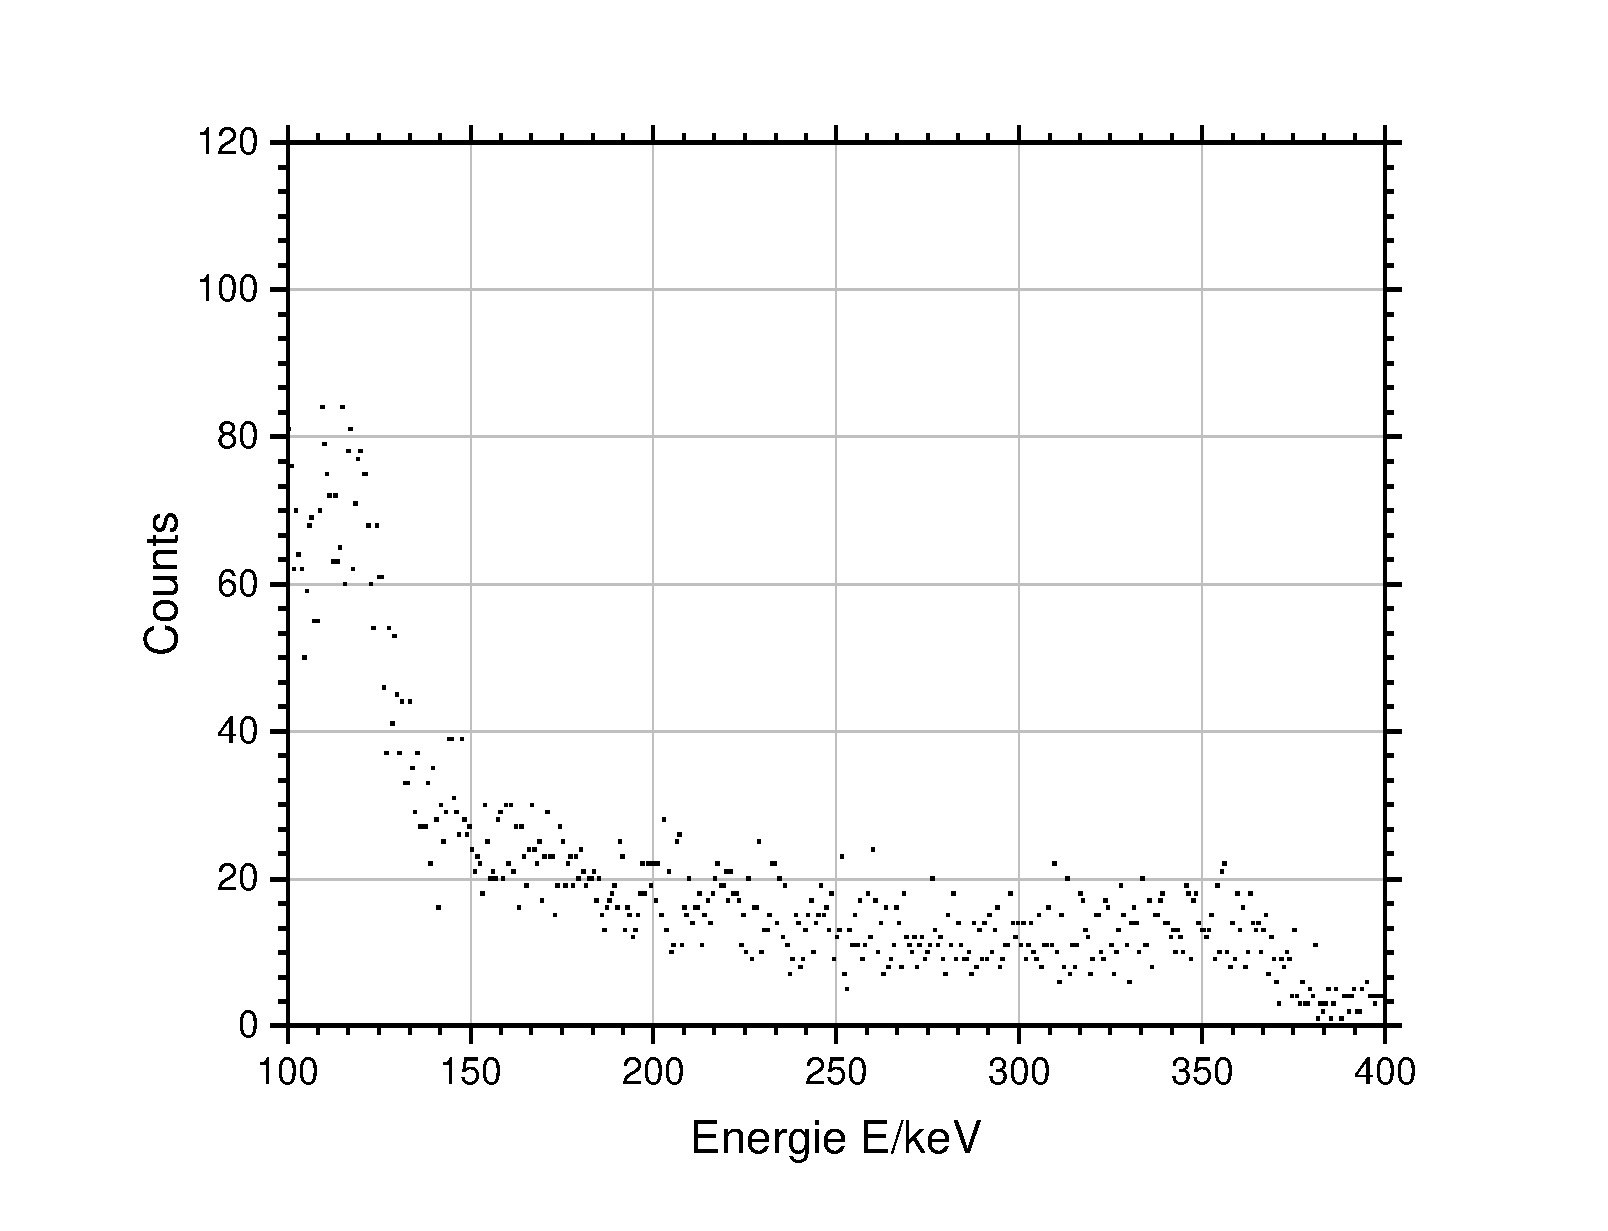
\includegraphics[width=\textwidth]{/home/tom/BE/Plots/Blei_ist_super.pdf}
\caption{Detailansicht des \(^{85}_{36}\mathrm{Kr}\)-Spektrums nach dem Durchgang durch Blei. Die Röntgenlinie von Blei ist nicht mit dargestellt.}
\end{figure} 
Der Verlauf folgt der Compton-Verteilung; die Compton-Kante ist bei etwa \(E\approx 370\,\mathrm{keV}\) deutlich zu erkennen. Die geringe Anzahl an Ereignissen spricht für die hohe Abschirmfähigkeit von Blei. Die Messung dieses Spektrums hat über eine Stunde gedauert, während die anderen Messungen nur jeweils fünf bis fünfzehn Minuten in Anspruch nahmen.
    % Bibliographie/Literaturverzeichnis
    \begin{thebibliography}{9}

    \bibitem{Anleitung}	
    Versuchsanleitung Beta-Spektrometrie (BE).Fortgeschrittenen-Praktikum im Studiengang Physik. 2015.
\end{thebibliography}
% Ende Dokument
\end{document}
